% !TeX root = ../../main.tex
\begin{flushright}
\end{flushright}\chapter{Gas preparation and spin control}

\section{\text{$^{87}\text{Sr}$} Properties and interest}

Strontium is an alkaline-earth-like element with several stable isotopes well documented in the literature (e.g., \cite{reschovsky_narrow-line_2018, zelevinsky_narrow_2006, blatt_measurement_2011, borkowski_mass_2014, KillianBEC}). The majority of these isotopes are bosonic ($^{88}\text{Sr}$, $^{86}\text{Sr}$, and $^{84}\text{Sr}$) with zero nuclear spin ($I=0$). 

In our work, we focus on the fermionic isotope $^{87}\text{Sr}$, which has a natural abundance of $7.0\%$. In contrast to its bosonic counterparts, $^{87}\text{Sr}$ possesses a large nuclear spin $I=9/2$, providing access to rich multi-level quantum dynamics ($SU(N)$ manifolds).

In the ground state $^1S_0$, the total electronic angular momentum is zero ($J=0$), making the atomic state almost insensitive to stray magnetic field fluctuations—a major advantage for mitigating environmental decoherence. However, this absence of an electronic magnetic moment also implies that magnetic fields alone cannot drive direct spin transitions via standard Zeeman manipulation. Specific optical techniques must therefore be developed to circumvent this limitation.

Furthermore, the decoupling between the nuclear spin and the electronic shell in the ground state leads to an $SU(N)$ collisional symmetry: the elastic scattering properties are strictly independent of the nuclear spin state $m_F$. The spin manipulation techniques developed by our group \cite{litvinov_measuring_2021} exploit this symmetry to yield a highly controllable quantum system whose internal spin dynamics remain decoupled from the spatial dynamics of the cloud once thermalized.

Preparation of the cold gas follows the standard scheme of ultracold gas experiments.
For $t_{\text{BlueMot}} = 8.2~\text{s}$, 2D transverse cooling (TC) collimates atoms prior to a Zeeman slowing stage, followed by a blue Magneto-Optical Trap (MOT), operating on the broad $^1S_0 \rightarrow {}^1P_1$ transition (see Fig.~\ref{energy levels sr}). Following this blue stage, repumping light is applied for $t_{\text{Repump}} = \text{\hl{time}}$, swept across multiple hyperfine states of the $^3P_2 \rightarrow {}^3D_2$ transition to recover approximately $25\%$ of the atoms trapped in the metastable $^3P_2$ state. The atoms are then cooled to temperatures close to $T = \text{\hl{temperature}}$ by a dynamic red MOT for $t_{\text{Red}}^{\text{tot}} = \text{\hl{time}}$ on the narrow $^1S_0 \rightarrow {}^3P_1$ transition. Finally, the gas is loaded and evaporated inside an Optical Dipole Trap (ODT).

\begin{figure}[H]
    \centering
    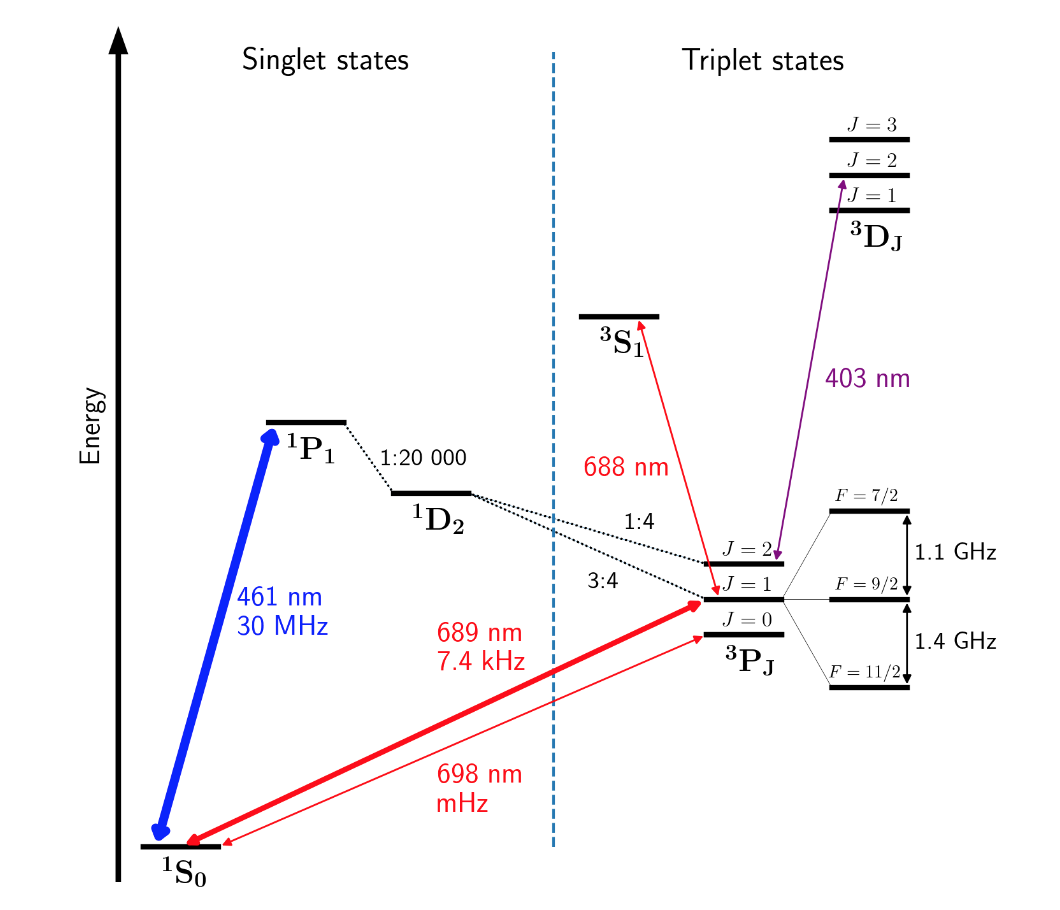
\includegraphics[width=1\linewidth]{Chapitres/Gas preparation and spin control/images/energy_levels_sr.png}
    \caption{Relevant low-lying electronic energy levels and optical cooling transitions for $^{87}\text{Sr}$.}
    \label{energy levels sr}
\end{figure}

In this chapter, I describe each stage of the cooling and loading process from a practical "user guide" perspective, concluding with an explanation of the spin manipulation schemes tailored to our experimental goals: coherent control of quantum systems, precision measurement, and photoassociation spectroscopy of $^{87}\text{Sr}$.

\section{Fermi gas preparation}
\hl{Ajouter ce qui est judicieux d'optimiser à chaque étape : nombre d'atomes, $T$, $T/T_F$, nombre d'atomes final chargé à chaque étape, vitesse.}

Solid strontium is vaporized in an oven heated to $490^\circ\text{C}$, outputting an atomic beam through a cluster of fine capillaries that provide initial spatial collimation.

\subsection{Blue optical setup}
The first cooling stages operate on the main $^1S_0 \rightarrow {}^1P_1$ transition using a master-slave laser architecture (see Fig.~\ref{fig:intro-chaine-bleue}). The master laser is an Extended-Cavity Diode Laser (ECDL, New Focus Vortex) frequency-stabilized via saturated absorption spectroscopy on $^{88}\text{Sr}$ \cite{bataille_realisation_nodate}. It seeds three high-power slave laser diodes, forcing them to inherit the master's narrow linewidth and central frequency while delivering the high output power needed for the cooling beams. This stage brings the atomic beam to a mean longitudinal velocity of \hl{$v$} at an equivalent beam temperature of \hl{$T=$}.

\begin{figure}[H]
    \centering
    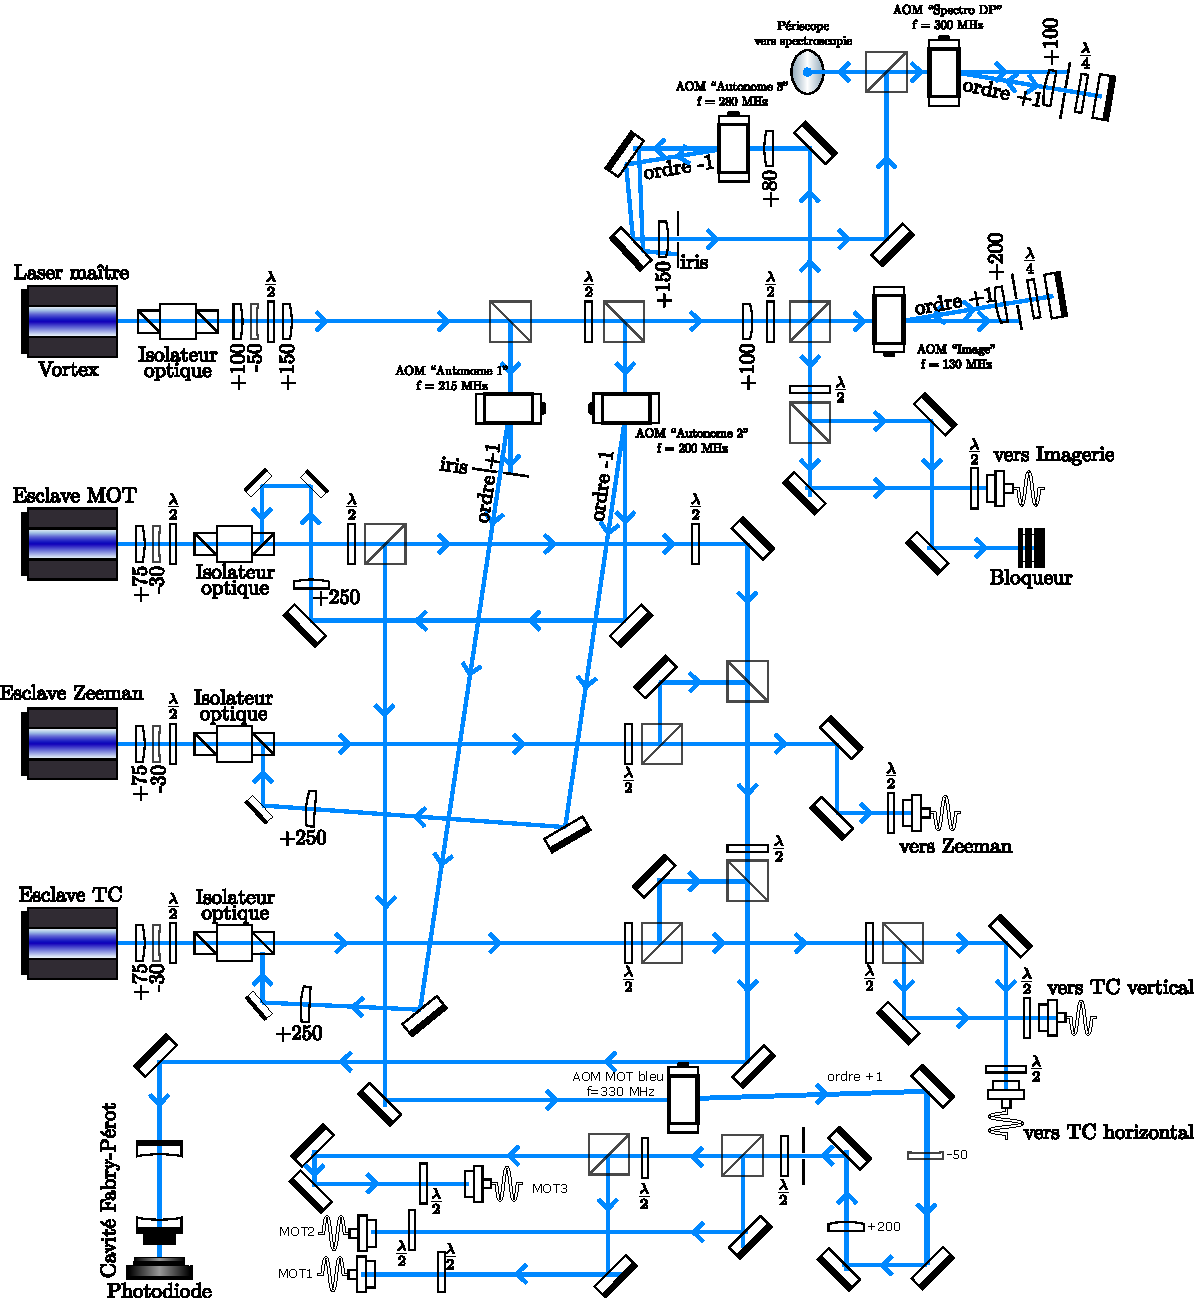
\includegraphics[width=1\linewidth]{Chapitres/Gas preparation and spin control/images/chaine_bleue_actualisée.pdf}
    \caption{Optical layout of the $461~\text{nm}$ blue laser system for transverse cooling, Zeeman slowing, and blue MOT.}
    \label{fig:intro-chaine-bleue}
\end{figure}

\hl{Ajouter schémas des fréquences.}

\subsection{Transverse cooling}

Following extraction from the oven capillaries, the atomic beam is collimated using 2D transverse cooling (TC). This stage employs two orthogonal pairs of counter-propagating laser beams perpendicular to the main longitudinal atomic propagation axis ($z$-axis), reducing the transverse velocity spread $v_\perp$ via photon recoil recoil momentum ($\hbar k_\perp$).

\subsubsection{Operating principle and radiation oressure}

The collimation relies on Doppler cooling. An atom moving with a transverse velocity $\vec{v}_\perp$ experiences a Doppler shift $\Delta_D = -\vec{k}_\perp \cdot \vec{v}_\perp$. As illustrated in Fig.~\ref{fig:doppler_shift}, atomic velocity classes observe shifted transition resonances centered at $\omega_0 \pm \vec{k}_\perp \cdot \vec{v}_\perp$. 
When the laser frequency is red-detuned ($\Delta < 0$) with respect to the atomic transition frequency ($\omega_0$), the atom preferentially absorbs photons from the counter-propagating beam, generating a net damping force.

\begin{figure}[H]
\centering
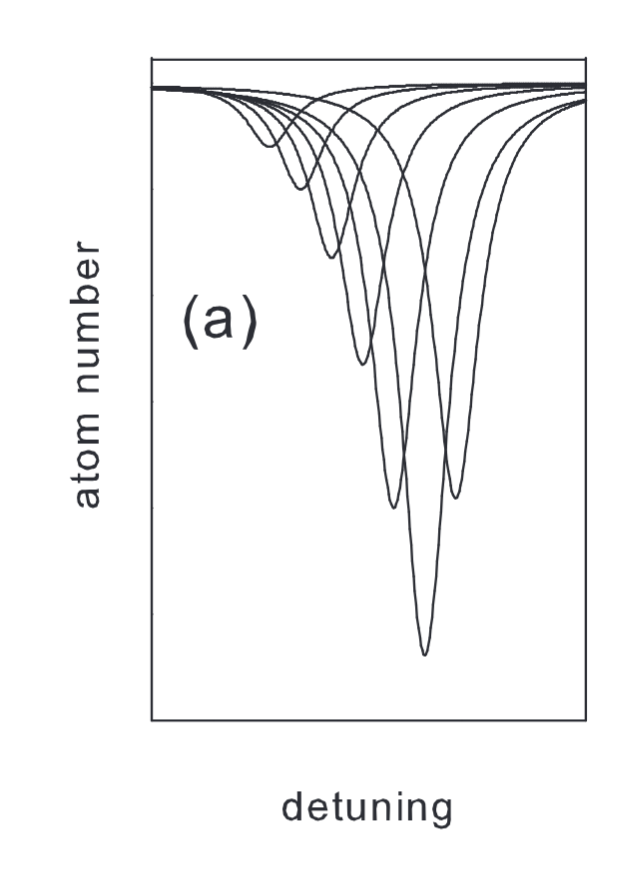
\includegraphics[width=0.5\linewidth]{Chapitres/Gas preparation and spin control/images/doppler_shift.png}
\caption{Illustration of Doppler cooling: velocity classes are shifted relative to the atomic resonance frequency $\omega_0$.}
\label{fig:doppler_shift}
\end{figure}

The underlying radiation pressure force acting on the atoms is given by:
\begin{equation}
F_{\text{rad}}(v_\perp) = \frac{\hbar k_\perp \Gamma}{2} \frac{s}{1 + s + 4 \left( \frac{\Delta_{\text{eff}}(v_\perp)}{\Gamma} \right)^2}
\label{eq:radiation_pressure}
\end{equation}
where $\Gamma$ is the natural linewidth of the transition, $s = I/I_{\text{sat}}$ is the saturation parameter, and $\Delta_{\text{eff}} = \Delta - \vec{k}_\perp \cdot \vec{v}_\perp$ is the effective detuning ($\Delta = \omega_{\text{laser}} - \omega_0$). In the low-intensity limit ($s \ll 1$), standard Doppler cooling theory predicts a maximum damping force gradient at a detuning of $\Delta_{\text{eff}} = -\Gamma/2$.

\subsubsection{Experimental setup and laser configuration}

For this stage, we drive the broad-linewidth $^1S_0 \rightarrow {}^1P_1$ transition ($\Gamma / 2\pi = 30.5~\text{MHz}$, $I_{\text{sat}} \approx 40~\text{mW/cm}^2$). The laser frequency $f_{\mathrm{TC}}$ is generated by shifting the main blue master frequency using an acousto-optic modulator (AOM) driven at $f^{\mathrm{RF}}_{\mathrm{TC}}$:
\begin{equation}
f_{\mathrm{TC}} = f_{\mathrm{Blue,Master}} + f^{\mathrm{RF}}_{\mathrm{TC}}
\end{equation}

Due to anisotropic geometric constraints of our atomic beam, the intensity in the horizontal arm is set roughly three times higher than in the vertical arm, though both remain below saturation ($I \ll I_{\text{sat}}$) over an interaction area of approximately $10~\text{cm}^2$. The TC laser remains active throughout subsequent blue-cooling stages to ensure continuous atomic flux collimation.

\subsubsection{Detuning and power optimization}

While ideal two-level theory predicts an optimal detuning of $\Delta = -\Gamma/2$, experimental constraints alter this optimum:
\begin{itemize}
\item \textbf{Power limitations over large beam areas:} Operating near saturation ($I \sim I_{\text{sat}}$) would maximize the velocity capture range through power broadening. However, illuminating the $10~\text{cm}^2$ interaction area at saturation would require over $400~\text{mW}$ of optical power. Consequently, the system operates in the low-intensity regime ($I \ll I_{\text{sat}}$).
\item \textbf{Optimal detuning shift:} Experimental characterization reported in F. Faisant's thesis \cite{faisant_building_2024} demonstrated that maximum collimation efficiency (measured by downstream atom yield) is achieved at $\Delta = -\Gamma/4$ rather than $-\Gamma/2$, as shown in Fig.~\ref{felix faisant}. This plot also illustrates how the maximum gain improves with total beam power.
\end{itemize}

\begin{figure}[H]
\centering
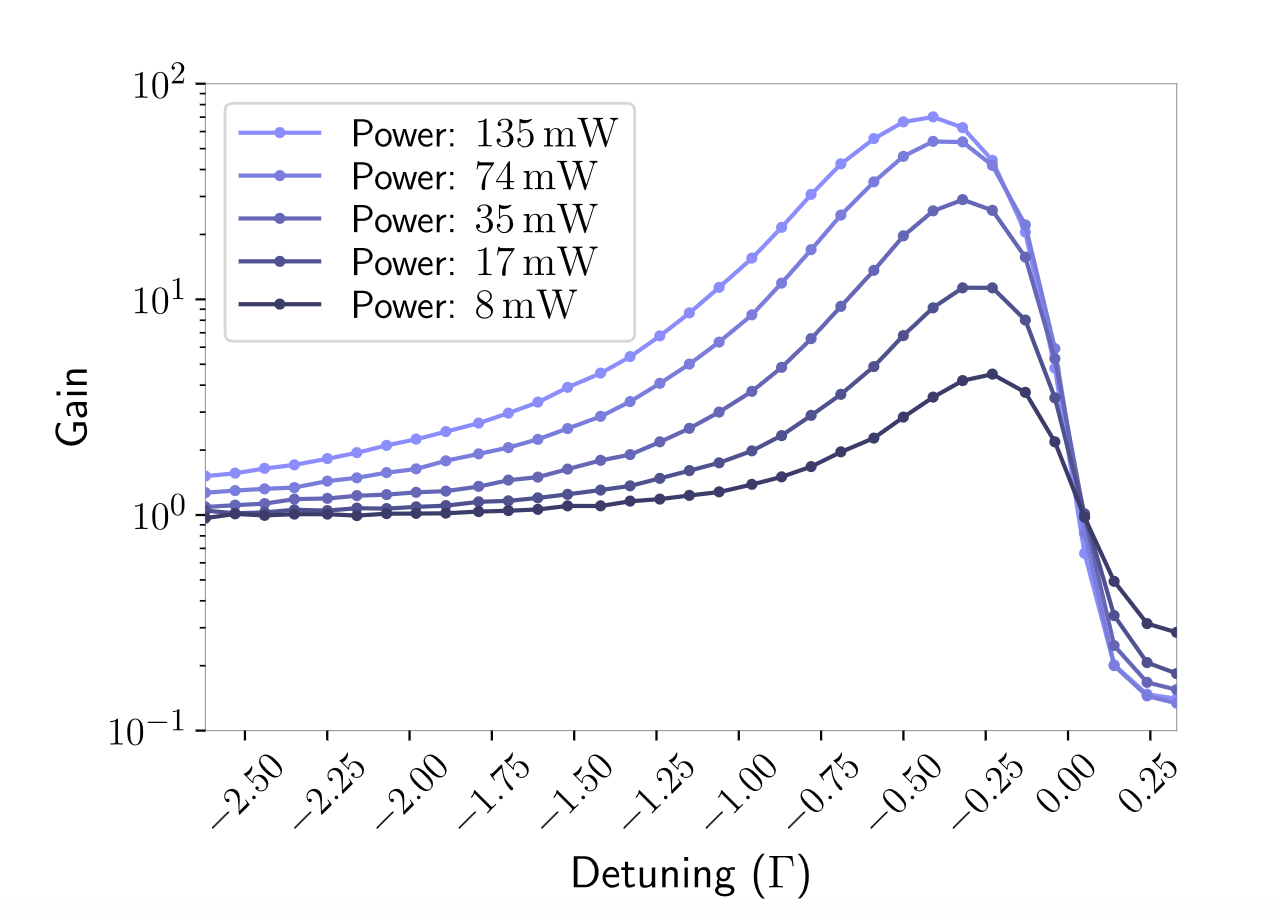
\includegraphics[width=0.8\linewidth]{Chapitres/Gas preparation and spin control/images/felix_faisant_these.png}
\caption{Transverse cooling performance as a function of laser detuning and power (adapted from \cite{faisant_building_2024}).}
\label{felix faisant}
\end{figure}

Future upgrades include replacing the current TC slave diode with a higher-power diode and re-optimizing $\Delta_{\text{eff}}$ to further enhance atom capture.\\
Following transverse collimation, the atomic beam enters the Zeeman slower stage along the main longitudinal axis.

\subsection{Zeeman cooling}
\hl{Valeur du gradient de champ B?}

Following transverse collimation, atoms are decelerated longitudinally using a Zeeman slower \cite{phillips_laser_1982}. The mechanism relies on a counter-propagating laser beam maintained on resonance with the decelerating atoms as they travel through a spatially varying magnetic field gradient $B(z)$ generated by a tapered solenoid.

To compensate for the decreasing Doppler shift $k v(z)$ as atoms slow down, the magnetic field $B(z)$ shifts the Zeeman sub-levels to satisfy the resonance condition along the entire deceleration path:
\begin{equation}
\Delta_{\text{eff}}(z) = \omega_{\text{laser}} - \omega_0 + k v(z) - \frac{\mu_B g_J B(z)}{\hbar} = 0
\end{equation}

At the slower entrance, atoms exhibit a mean velocity of $v_0 = 434~\text{m/s}$ \cite{Bataille2020}. As the field $B(z)$ drops toward zero near the main cell center to avoid disturbing downstream trapping, atoms above the capture velocity can pass through this zero-field zone. To capture these remaining fast atoms, supplementary coils with increasing radii produce an additional field gradient that shifts Zeeman levels back into resonance, ensuring deceleration down to the final capture velocity.

\subsection{Blue MOT}

The Magneto-Optical Trap (MOT) provides simultaneous spatial confinement and cooling. 

The blue MOT combines a magnetic quadrupole field (generated by anti-Helmholtz coils centered on the vacuum chamber) with three orthogonal pairs of counter-propagating $461~\text{nm}$ laser beams carrying opposite circular polarizations ($\sigma^+/\sigma^-$) \cite{phillips_laser_1998}. 

The position-dependent Zeeman shift breaks the spatial degeneracy of the sub-levels:
\begin{equation}
\Delta E(z) = - m_F g_F \mu_B B(z)
\end{equation}
Combined with red-detuned laser beams, this spatial shift creates a restoring force toward the trap center ($z = 0$) alongside the velocity-dependent radiation pressure force.

Gravity compensation and vertical spatial confinement are provided by the magnetic field gradient itself. Because the quadrupole coils produce a steeper gradient along their symmetry axis ($z$) than in the horizontal plane ($x, y$), half as much intensity is delivered along the vertical axis compared to the horizontal axes. This ratio achieves a balanced, quasi-spherical trap while minimizing power broadening and optical density effects.

During this stage, the cloud reaches the Doppler temperature limit \cite{dalibard_atomes_froids}:
\begin{equation}
k_B T_D = \frac{\hbar \Gamma_{^1S_0 \rightarrow {}^1P_1}}{2}
\end{equation}
Due to the broad linewidth of the $461~\text{nm}$ transition ($\Gamma/2\pi = 30.5~\text{MHz}$), this Doppler temperature ($T_D \approx 770~\mu\text{K}$) remains significantly higher than the single-photon recoil limit $T_r$.

\subsection{Repumper}

To sustain the blue MOT cycle, a repumping laser system is required: approximately $1$ out of every $150{,}000$ excitations to $^1P_1$ decays into the metastable $^3P_2$ state (lifetime $\tau \approx 500~\text{s}$) via the intermediate $^1D_2$ state. Without repumping, atoms become dark to the $461~\text{nm}$ light and are lost from the cooling cycle.

\subsubsection{Hyperfine structure of Strontium-87}
Because fermionic $^{87}\text{Sr}$ possesses a nuclear spin $I = 9/2$, its electronic states exhibit a rich hyperfine structure that must be addressed for efficient repumping.

Repumping is provided by a $403~\text{nm}$ external-cavity diode laser (TOPTICA). To address multiple $F$ hyperfine sub-levels (see Fig.~\ref{fig:intro-energy-levels-repumper}), the laser frequency is rapidly swept over a $3~\text{GHz}$ bandwidth.

\begin{figure}[H]
    \centering
    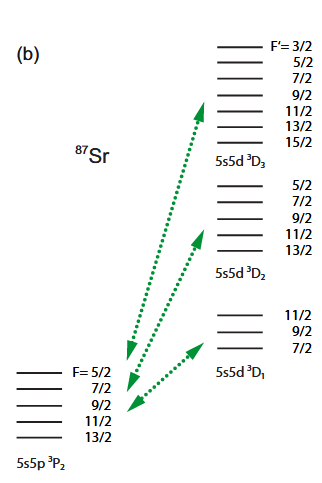
\includegraphics[width=0.4\linewidth]{Chapitres/Gas preparation and spin control/images/energy_levels_repumper.png}
    \caption{Energy level diagram of $^{87}\text{Sr}$ showing the primary $461~\text{nm}$ cooling transition and the $403~\text{nm}$ repumping pathway from $^3P_2$ to $^3D_2$.}
    \label{fig:intro-energy-levels-repumper}
\end{figure}

\subsubsection{Optimization of the repumper sweep}
The $^3P_2$ hyperfine levels are unequally populated during blue MOT decay due to their differing $g_F$ Landé factors, affecting their magnetic trapping efficiency \cite{stellmer_creation_2012}.

The repumper frequency scan range is optimized around $3~\text{GHz}$ to selectively cover the $F=11/2$ and $F=13/2$ states. Scanning a wider range reduces total atom recovery by decreasing the dwell time on these critical transitions. At the end of the blue MOT phase, the $461~\text{nm}$ beam is extinguished while the $403~\text{nm}$ repumper remains active for $\approx 200~\text{ms}$ at $I \approx 15~\text{mW/cm}^2$, returning trapped metastable atoms to the $^1S_0$ ground state before starting the red MOT.

\begin{figure}[H]
    \centering
    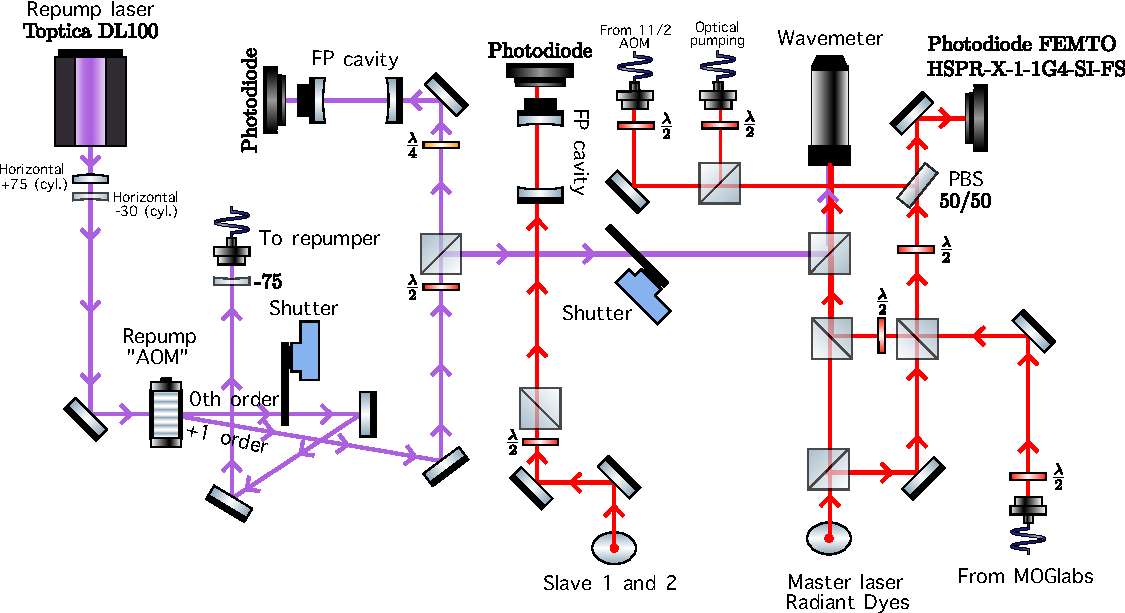
\includegraphics[width=1\linewidth]{Chapitres/Gas preparation and spin control/images/table_repumper.pdf}
    \caption{Summary of repumping beam frequencies and timing sequence.}
    \label{fig:intro-repompeur}
\end{figure}

\subsection{Red MOT}

\subsubsection{Optical setup}
Because the blue MOT temperature is bounded by $T_D \approx 770~\mu\text{K}$, further cooling requires transferring atoms to the narrow intercombination transition $^1S_0 \rightarrow {}^3P_1$ at $689~\text{nm}$ ($\Gamma = 2\pi \times 7.4~\text{kHz}$).

For this transition, the formal Doppler limit ($T_D = \hbar \Gamma / 2 k_B = 179~\text{nK}$) falls below the single-photon recoil limit ($T_r = \hbar^2 k^2 / m k_B = 283~\text{nK}$). Consequently, the ultimate red MOT temperature is bounded by the photon recoil limit.

The $689~\text{nm}$ light is generated by a commercial laser locked to an ultra-stable optical cavity. The frequency is offset-shifted by \hl{$f = -600\text{ MHz}$} using a first AOM before injection into a master-slave system. A double-pass AOM fine-tunes the frequency before splitting into three spatial counter-propagating beam pairs.

\begin{figure}[H]
    \centering
    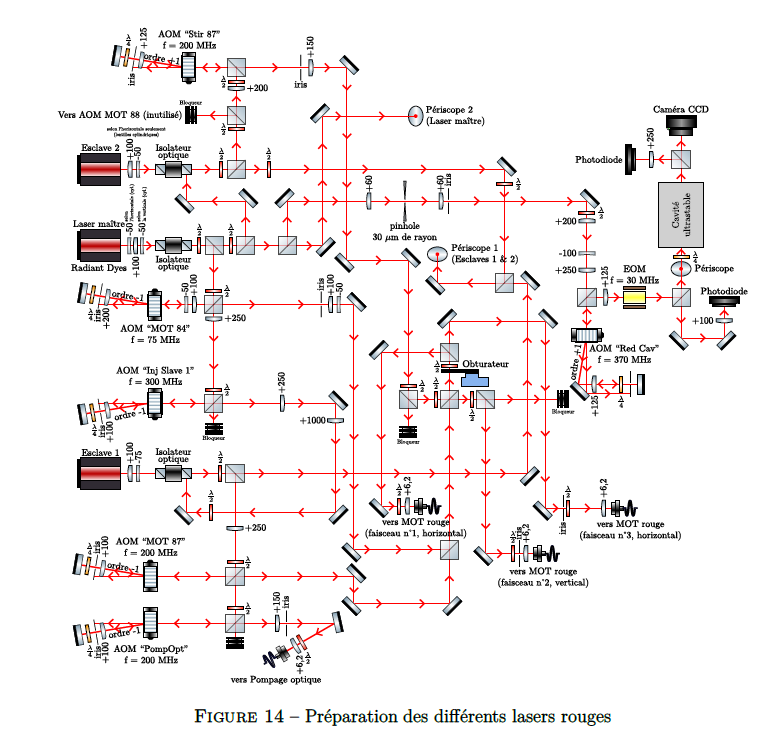
\includegraphics[width=1\linewidth]{Chapitres/Gas preparation and spin control/images/chaine_rouge_vieille.png}
    \caption{Optical layout of the $689~\text{nm}$ laser cooling system.}
    \label{fig:intro-chaine-rouge}
\end{figure}

\subsubsection{Broadband MOT}
At the end of the blue MOT, the atomic cloud's spatial spread ($\sigma = \text{\hl{value}}$) and thermal energy exceed the capture velocity of a single-frequency $689~\text{nm}$ MOT.

To capture these thermal atoms, a broadband MOT is implemented on the $^1S_0 (F=9/2) \rightarrow {}^3P_1 (F=11/2)$ transition under a weak magnetic field gradient. The laser spectrum is artificially broadened by applying a sawtooth frequency modulation red-detuned from resonance. As the cloud cools and compresses, both the modulation amplitude $\Delta f$ and total optical power are ramped down.

\subsubsection{Stirring laser}
Simultaneously, a "stirring" laser beam is applied to redistribute populations among magnetic sub-levels. Because the $F=9/2 \rightarrow F=11/2$ cooling transition contains weak or non-absorbing Zeeman sub-states at the cloud edges, atoms accumulated in these states experience reduced radiation pressure and escape the trap (Fig.~\ref{fig:intro-need-for-stir}).

The stirring laser drives the $^1S_0 (F=9/2) \rightarrow {}^3P_1 (F=9/2)$ transition to optically pump and randomize $m_F$ populations (Fig.~\ref{fig:intro-randomisation}), restoring efficiency to the cooling cycle.

\begin{figure}[H]
    \centering
    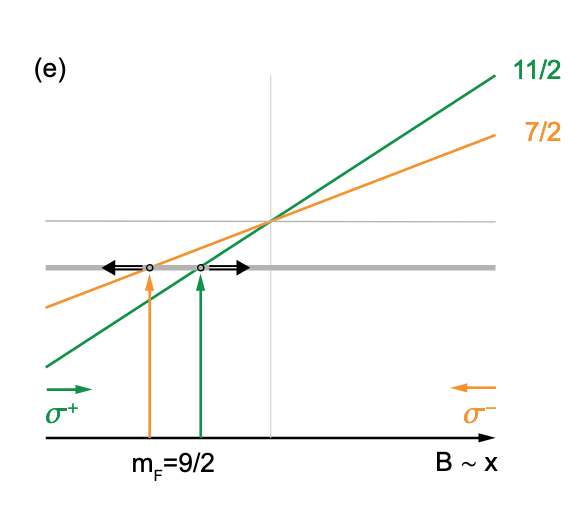
\includegraphics[width=0.7\linewidth]{Chapitres/Gas preparation and spin control/images/need_for_stir.png}
    \caption{Mechanism of population trapping in extreme Zeeman sub-states during the red MOT.}
    \label{fig:intro-need-for-stir}
\end{figure}

\begin{figure}[H]
    \centering
    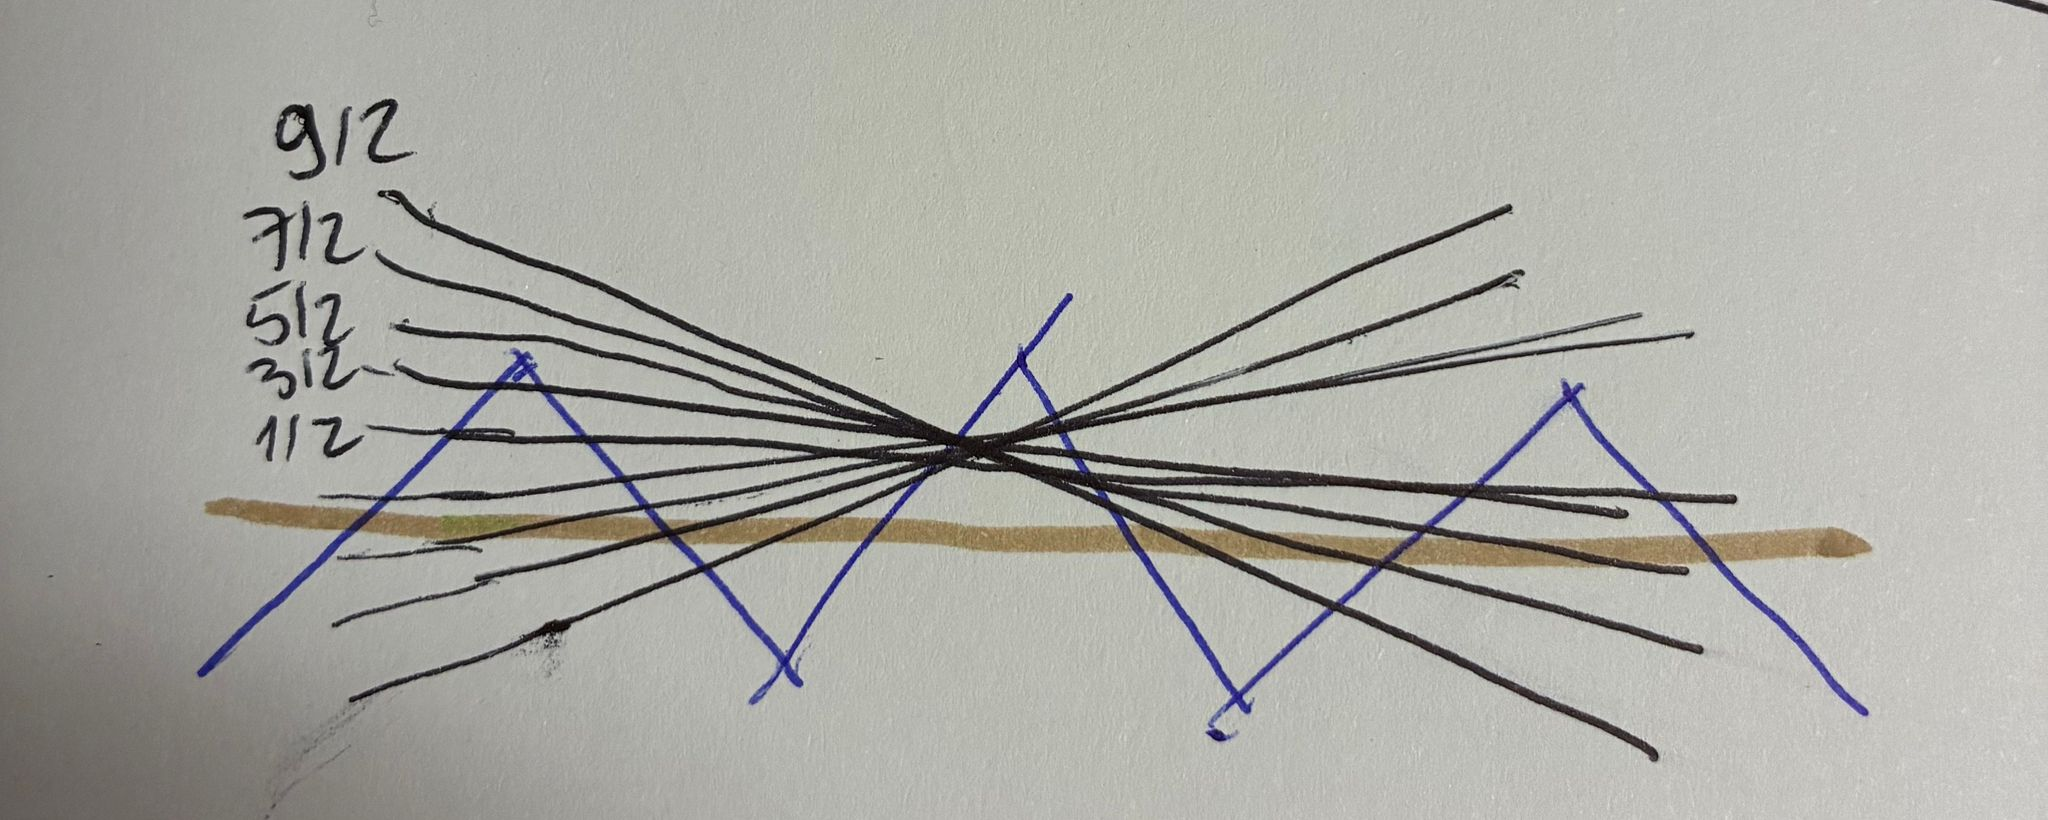
\includegraphics[width=0.7\linewidth]{Chapitres/Gas preparation and spin control/images/randomisation.jpeg}
    \caption{Randomization of $m_F$ populations induced by the $689~\text{nm}$ stirring laser.}
    \label{fig:intro-randomisation}
\end{figure}

Because the narrow linewidth of the intercombination transition ($\Gamma = 2\pi \times 7.4~\text{kHz}$) strictly bounds the saturation radiation pressure force to a theoretical maximum of $F_{\text{max}} = \hbar k \Gamma / 2 \approx 1.6~mg$, gravity plays a critical role during this stage. 

In practice, to minimize power broadening and reach microkelvin temperatures, the red MOT operates at low saturation parameters ($s \lesssim 1$). Under these conditions, a symmetric beam intensity would yield a radiation pressure force weaker than gravity ($F_{\text{rad}} < mg$), causing the atoms to fall out of the trap. To overcome this limitation, a significantly higher intensity is delivered specifically along the vertical axis to maintain $F_{\text{rad}} > mg$ and support the cloud against gravity, while lower intensities are maintained on the horizontal axes to prevent unnecessary power broadening and transverse heating.
\subsubsection{Narrowband MOT (Single-frequency MOT)}
Once the cloud is sufficiently cold, frequency modulation is switched off to operate a single-frequency (monofrequency) MOT. This stage reduces the temperature to $1\text{--}2~\mu\text{K}$ (near the recoil limit) with a peak density of $n = \text{\hl{value}}$ and an RMS width of $\sigma = \text{\hl{value}}$.

\begin{figure}[H]
    \centering
    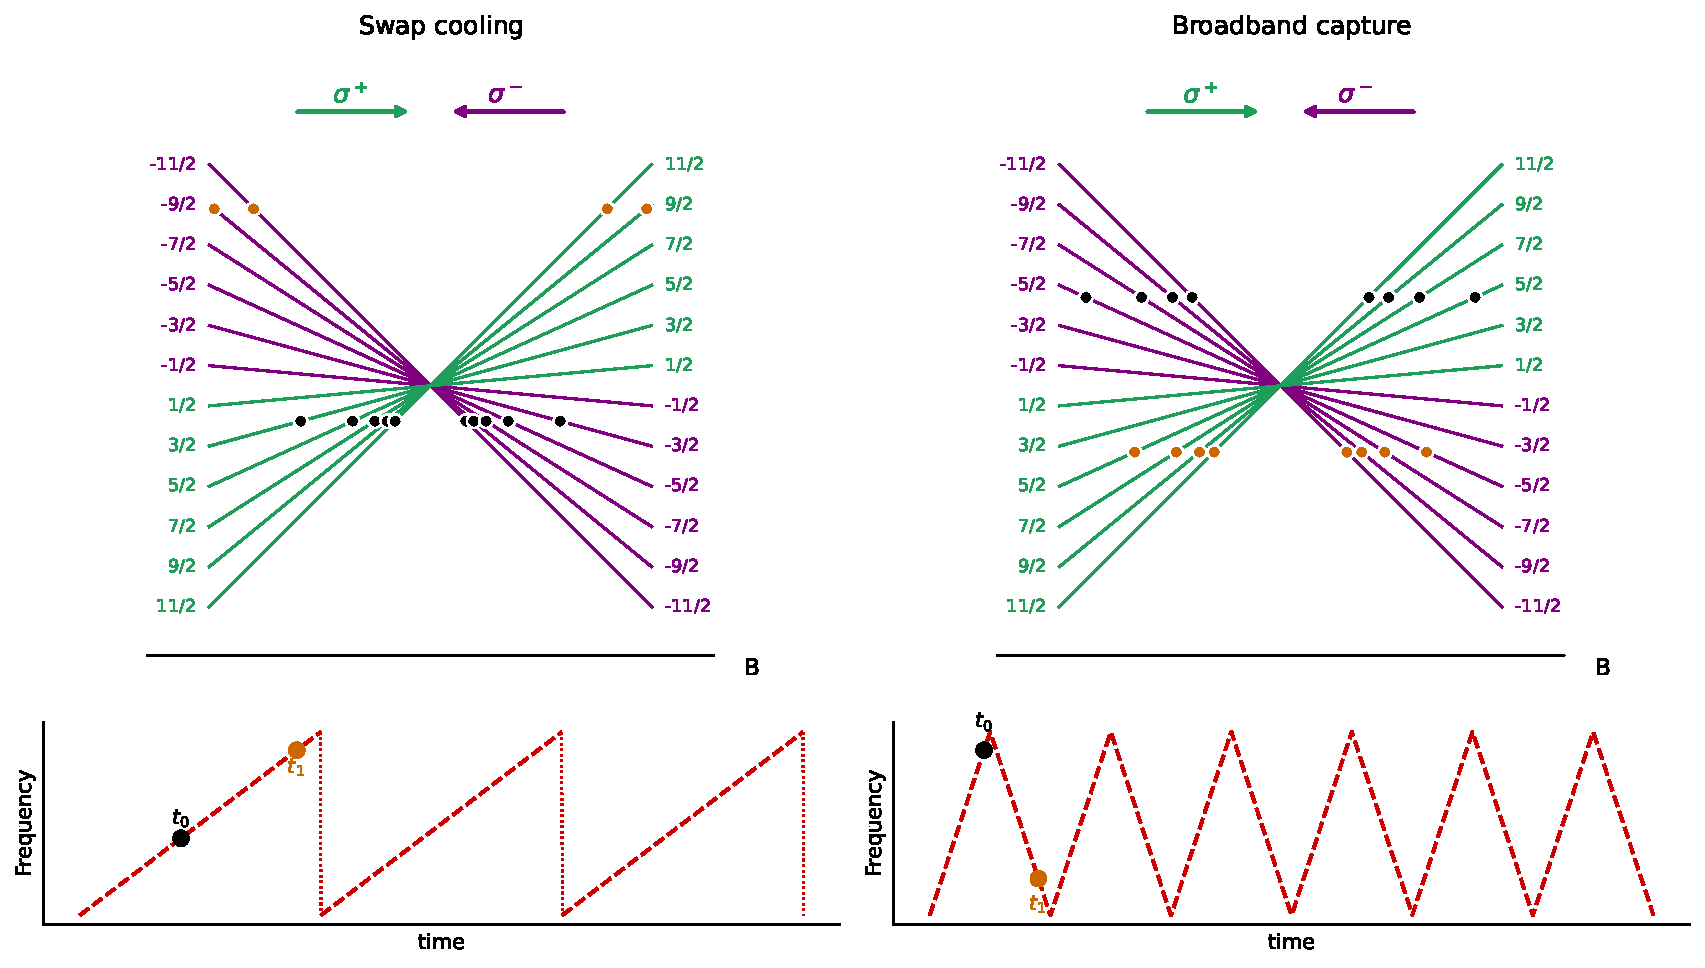
\includegraphics[width=1\linewidth]{Chapitres/Gas preparation and spin control/images/red_MOT_in_3_steps.pdf}
    \caption{Sequential stages of the $689~\text{nm}$ red MOT: broadband capture, compression, and single-frequency cooling (adapted from \cite{StellmerThesis}).}
    \label{fig:intro-red-mot-3-steps}
\end{figure}

\subsubsection{Optimization of narrowband MOT Parameters}

Cooling efficiency during the single-frequency stage depends on precise frequency, intensity, and timing parameters:
\begin{itemize}
    \item \textbf{Broadband modulation amplitude:} The initial sweep covers $\Delta f = 3~\text{MHz}$ at the RF source to capture the Doppler distribution from the blue MOT.
    
    \item \textbf{Intensity ramp and power broadening:} High intensity provides a deep trap for initial capture, but causes power broadening ($\Gamma_{\text{eff}} = \Gamma \sqrt{1 + I/I_s}$), raising the achievable Doppler limit. For single-frequency cooling, intensity is adiabatically ramped down over $45~\text{ms}$ to reduce power broadening while maintaining sufficient force to support the cloud against gravity.
    
    \item \textbf{Detuning optimization:} Setting the laser too close to resonance causes re-heating via photon re-absorption in dense clouds. During the single-frequency MOT, the laser detuning is fixed at $\Delta f = -600~\text{kHz}$, optimized experimentally to minimize final cloud temperature.
    
    \item \textbf{Magnetic field bias and quantization axis:} To preserve spin polarization, the magnetic field is never allowed to cross zero during transitions between cooling phases. Maintaining non-zero bias components along at least two orthogonal directions (e.g., $|B_x|$ and $|B_y|$) preserves the quantization axis and prevents spin depolarization.
\end{itemize}

\subsection{Optical Dipole Trap (ODT) and evaporative cooling}

\subsubsection{Loading the crossed ODT}
The final cooling stage before optical trapping consists in transferring the atoms into an Optical Dipole Trap (ODT) operating at $1070~\text{nm}$, followed by forced evaporative cooling.

Atoms are adiabatically loaded into the ODT while decreasing the intensity of the single-frequency $689~\text{nm}$ red MOT during a ramp lasting \hl{temps, intensity ramp}. From second-order perturbation theory, the light shift experienced by the energy levels yields the optical dipole potential:
\begin{equation}
    U_{\text{dip}} = -\frac{\hbar|\Omega|^2}{4\bar{\Delta}}
\end{equation}
\cite{litvinov_these}, where $1/\bar{\Delta} = 1/(\omega_{\text{laser}} - \omega_{\text{atomic}}) - 1/(\omega_{\text{laser}} + \omega_{\text{atomic}})$ is the effective detuning factor, and $\Omega^2 = \frac{\Gamma^2}{2}\frac{I}{I_{\text{sat}}}$ is the Rabi frequency.

As seen from these expressions, the AC Stark shift induced by the dipole laser is state-dependent. As illustrated in Fig.~\ref{fig:intro-odt-loading}, the potential estimated in \cite{litvinov_these} is deeper for the ground state $^1S_0$ ($U_{\text{dip}}(^1S_0) \simeq -1.5~\text{MHz}$) than for the excited state $^3P_1$ ($U_{\text{dip}}(^3P_1) \simeq -1.2~\text{MHz}$) at the center of the trap, resulting in a differential red-shift of the $^1S_0 \rightarrow {}^3P_1$ transition.

This differential shift creates a localized spatial resonance condition: atoms at the center of the trap remain in resonance with the red MOT beams, where they are continuously cooled and trapped. Conversely, energetic atoms at the periphery experience a negligible light shift and remain blue-detuned from the local resonance, preventing unwanted re-heating.

\begin{figure}
    \centering
    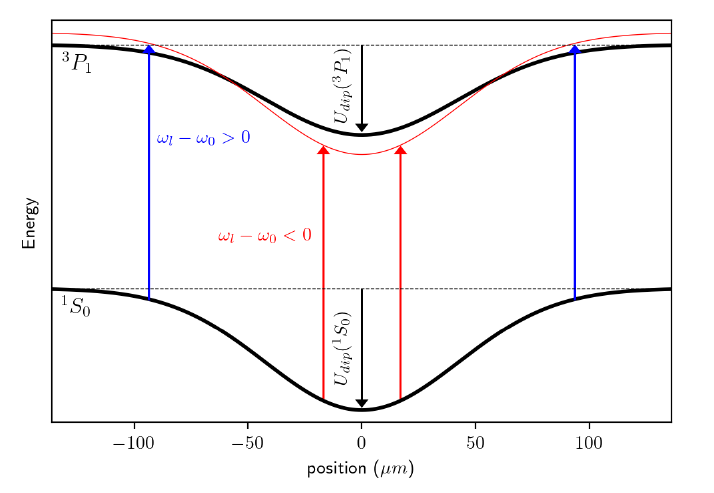
\includegraphics[width=0.7\linewidth]{Chapitres/Gas preparation and spin control/images/ODT_loading.png}
    \caption{Simulation extracted from \cite{litvinov_these}. Principle of localized $689~\text{nm}$ MOT loading inside the crossed optical dipole trap due to the differential AC Stark shift between $^1S_0$ and $^3P_1$.}
    \label{fig:intro-odt-loading}
\end{figure}

Following loading, forced evaporative cooling is performed to reach deep Fermi degeneracy, down to temperatures on the order of $T =, T/T_F=$ \hl{calculer avec les valeurs du temps d'husain}. Evaporative cooling is achieved by adiabatically lowering the trap depth: the most energetic atoms overcome the potential barrier and escape the trap, while the remaining ones re-thermalize to lower temperatures via elastic collisions (Fig.~\ref{fig:evap}).

The results presented in the following two chapters were obtained with an atomic cloud located at the intersection of a horizontal beam, called the ``Reservoir'' (waist $w_0^H = 150~\mu\text{m}$), and a vertical beam, called the ``Dimple'' (waist $w_0^V = 80~\mu\text{m}$). The vertical beam axis is tilted at an angle of $\simeq 30^\circ$ relative to the vertical to facilitate the escape of the hottest atoms from the trap.

In Chapter 2, the horizontal arm is tilted by $\simeq 1^\circ$. For the photoassociation results in Chapter 3, this tilt was canceled: \hl{ajouter des arguments et refs pour motiver ça}.

\begin{figure}[H]
    \centering
    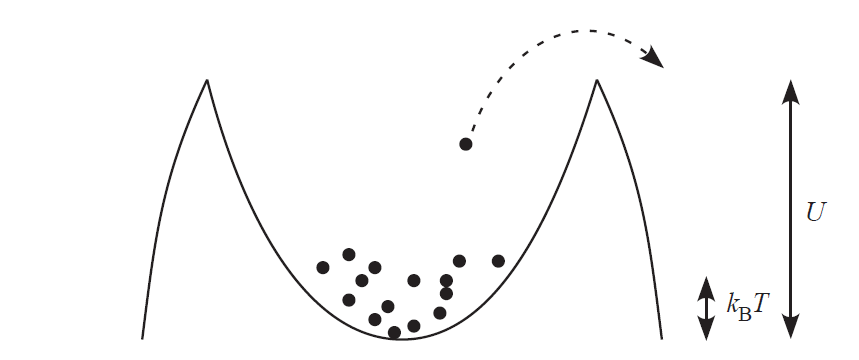
\includegraphics[width=0.7\linewidth]{Chapitres/Gas preparation and spin control/images/evaporative_cooling.png}
    \caption{Evaporative cooling mechanism in an inclined crossed optical dipole trap, illustrating the escape of high-energy atoms and subsequent re-thermalization.}
    \label{fig:evap}
\end{figure}

\subsubsection{Optimization of the evaporation ramps}

For a degenerate Fermi gas, the key parameter to optimize is the phase-space density (PSD), which scales as $\text{PSD} \propto N\bar{\omega}^3/T^3$, where $N$ is the atom number, $\bar{\omega}$ the geometrically averaged trap frequency, and $T$ the temperature. While both arms of the dipole trap influence these parameters, their main physical contributions differ:

\begin{itemize}
    \item \textbf{Tight vertical beam (``Dimple''):} Writing the atom number as $N = nV$ (where $n$ is the spatial density and $V$ the trap volume), the elastic collision rate scales as $\Gamma_{\text{el}} = n\sigma_{\text{el}}v_{\text{th}}$. The tightly focused waist of the dimple beam mainly dictates the local confinement, thereby enhancing collision rates for fast re-thermalization. Moreover, ramping down the dimple intensity directly lowers the effective trap depth, setting the final temperature $T$ of the cloud.
    
    \item \textbf{Broad horizontal beam (``Reservoir''):} Due to its large waist and capture volume, the reservoir beam primarily serves to maximize the initial atom number $N$ loaded from the MOT. While modifying its intensity also reshapes the cloud and affects thermalization dynamics, its primary role remains maintaining a high-capacity atomic reservoir.
    
    \item \textbf{Ramp duration and adiabaticity:} The duration and adiabaticity of the evaporative ramps depend on the targeted state. Short evaporations are preferred when aiming solely for a large atom number at moderate temperatures when it is necessary to detect atom number fluctuations, such as for our experiments on photoassociation (see Chapt.3). 
    Conversely, reaching deep quantum degeneracy requires a multi-stage ramp lasting approximately \hl{5 seconds} which was necessary for the results of Chapt.2.
\end{itemize}
For further details on loading atoms into the optical crossed dipole trap, the reader is referred to the thesis of A. Litvinov~\cite{litvinov_these}. An additional optical lattice, formed by a $1064~\text{nm}$ ALS laser, was initially implemented to enhance the phase-space density (PSD) of the atomic cloud prior to forced evaporative cooling. While this configuration was employed for the experiments presented in Chapter~2, it was subsequently discarded due to intensity fluctuations in the laser that induced significant heating.
\subsubsection{Optical setup}

\begin{figure}[H]
    \centering
    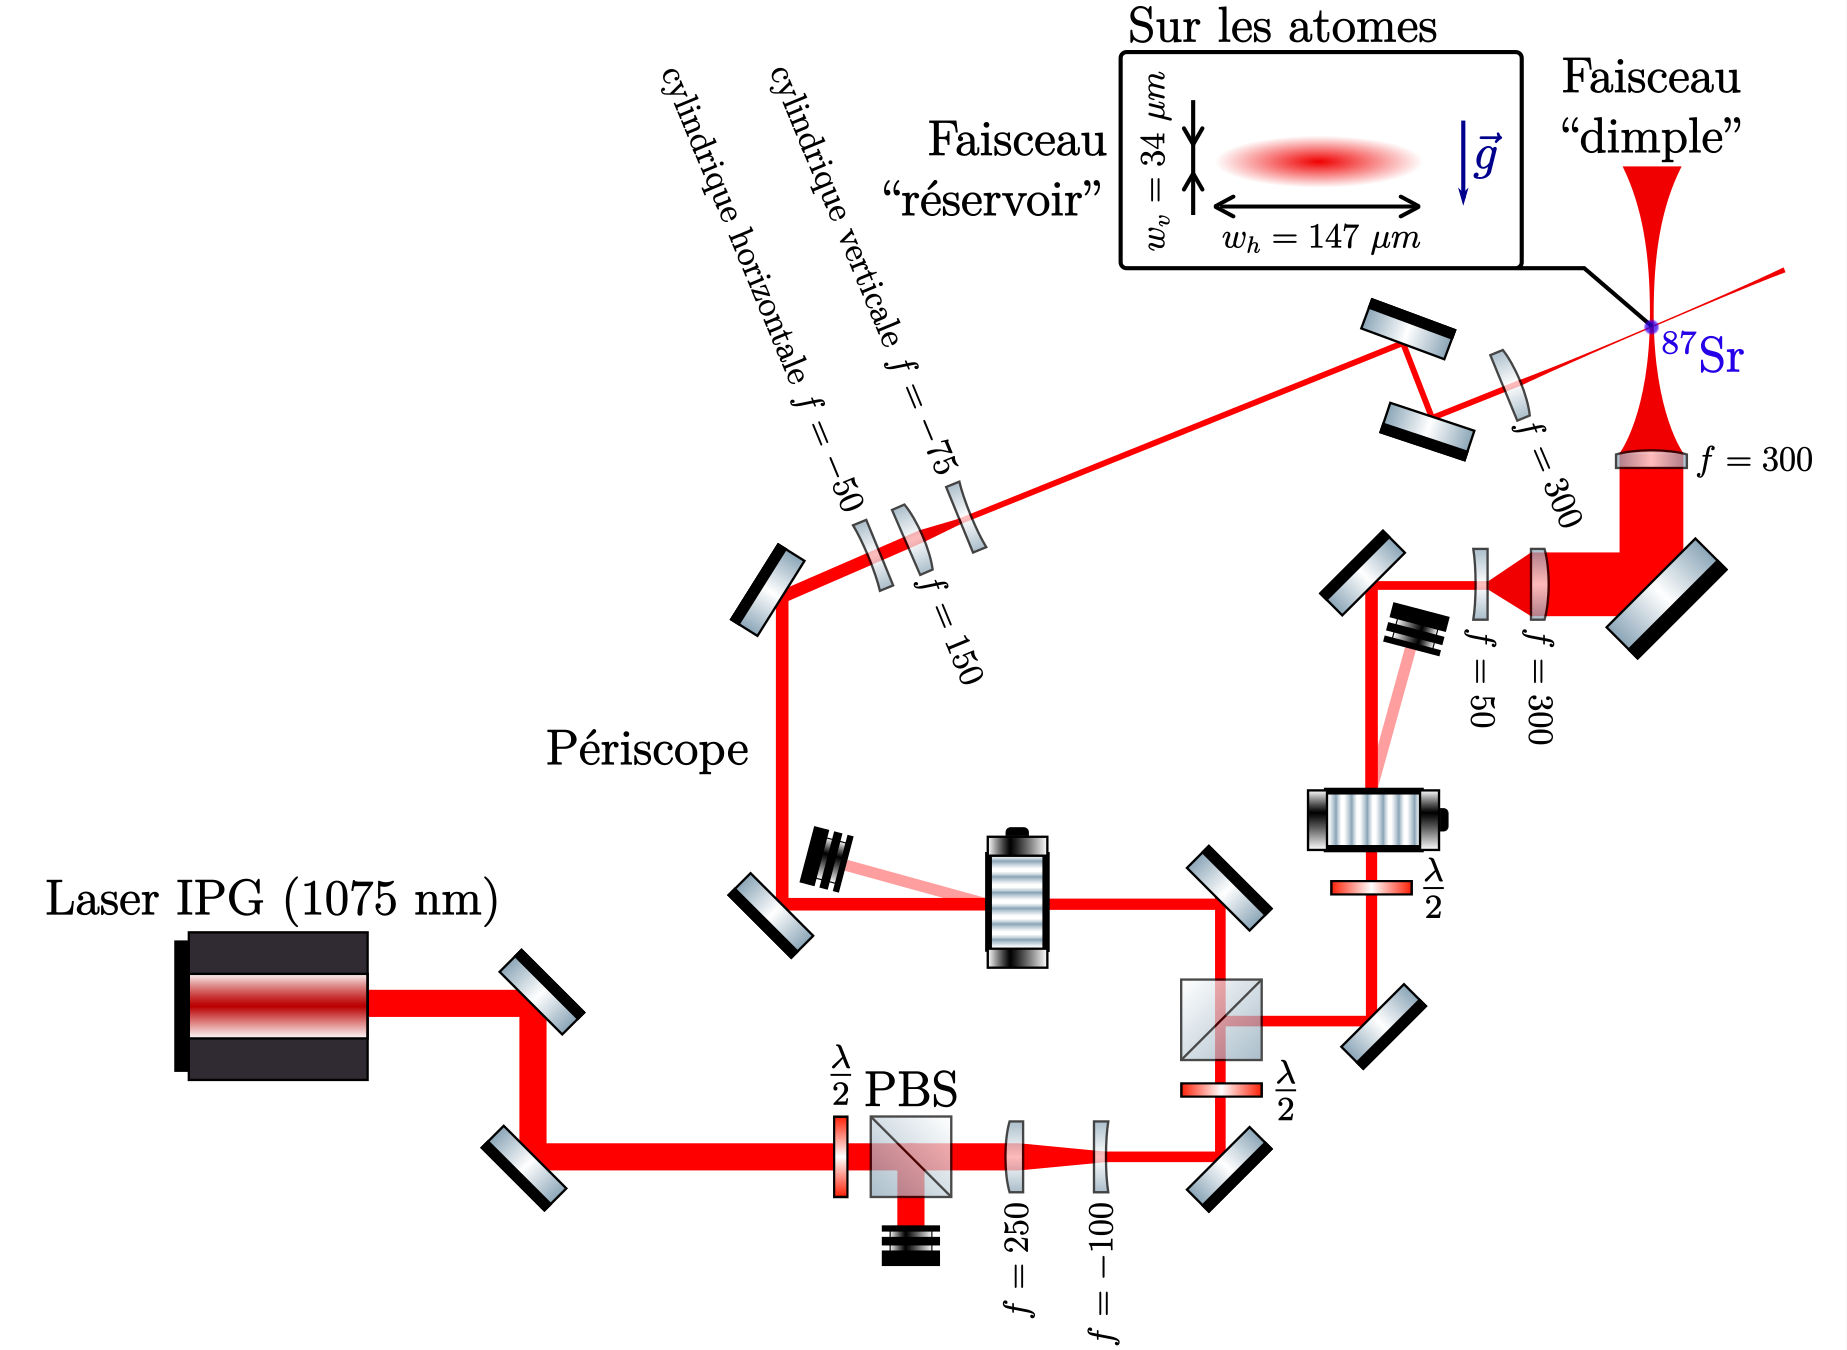
\includegraphics[width=1\linewidth]{Chapitres/Gas preparation and spin control/images/1.30_dipole_trap(1075)_setup.png}
    \caption{Optical layout of the $1075~\text{nm}$ crossed dipole trap laser system.}
    \label{fig:odt}
\end{figure}

\section{Spin Selection}

\subsection{Optical Pumping}
Optical pumping is implemented prior to the final evaporation stages to prepare the atomic gas in a tailored mixture of nuclear spin states ($m_F$). Due to the $SU(N)$ symmetry of $^{87}\text{Sr}$, elastic $s$-wave collisions between identical fermions in the same $m_F$ state are forbidden by the Pauli exclusion principle. Therefore, at least two distinct spin components must be present to enable elastic collisions and ensure efficient re-thermalization during evaporative cooling. Furthermore, $SU(N)$ symmetry guarantees that elastic collisions conserve the nuclear spin state, preventing spin-exchange collisions during evaporation.

To perform state preparation, a bias magnetic field of $6.05 \pm 0.05~\text{G}$ is applied to lift the degeneracy of the $^3P_1, F = 11/2$ hyperfine sub-levels via the linear Zeeman effect. The cloud is illuminated by a $\sigma^-$-polarized optical pumping beam tuned to the $^1S_0 (F=9/2) \rightarrow {}^3P_1 (F=11/2)$ transition. Its frequency is defined as:
\begin{equation}
f_{11/2} = f_{\text{Radiant Dyes}} \pm f_{\text{Slave 1}}^{\text{RF}} + f_{11/2}^{\text{RF}}
\end{equation}
The laser frequency is swept across \hl{ajouter amplitude rampe} the targeted $^3P_1, F = 11/2, m_F'$ sub-levels to deplete specific ground-state populations in $^1S_0, F=9/2, m_F$. Governed by electric dipole selection rules ($\Delta m_F = 0, \pm 1$), spontaneous emission redistributes the excited atoms into adjacent lower ground-state sub-levels, resulting in a progressive accumulation in the target spin states.

\hl{Note: Add efficiency comments, pulse duration $t = \text{value}$, and intensity $I = \text{value}$.}

To prepare a specific mixture (e.g., a 2-spin mixture), unwanted spin populations are sequentially pumped out. One spin component, typically $m_F = -9/2$, is intentionally retained alongside the target mixture to maintain two-body elastic collisions for thermalization during evaporation. Once evaporative cooling is complete, this auxiliary component is selectively removed using a short \textbf{'blast'} pulse. Under $\sigma^-$ excitation on the $F=9/2 \rightarrow F'=11/2$ transition, the $m_F = -9/2$ state couples exclusively to $m_F' = -11/2$. Because no $m_F = -11/2$ ground state exists, spontaneous emission from $m_F' = -11/2$ can only decay back to $m_F = -9/2$, forming a closed cycling transition. The resulting continuous photon scattering exerts a strong radiation pressure that expels the $m_F = -9/2$ population from the trap without disturbing the target mixture.

\begin{figure}[H]
    \centering
    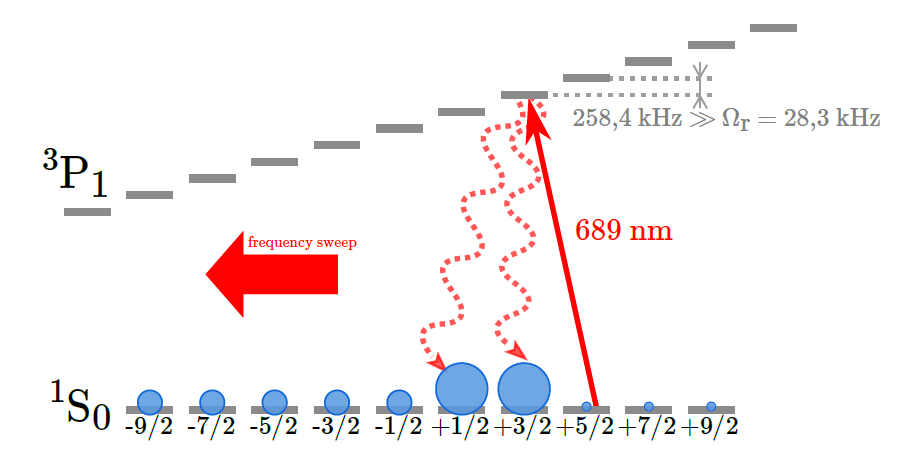
\includegraphics[width=1\linewidth]{Chapitres/Gas preparation and spin control/images/optical_pumping.png}
    \caption{Optical pumping scheme on the $^1S_0 (F=9/2) \rightarrow {}^3P_1 (F=11/2)$ transition used to prepare a specific nuclear spin mixture.}
    \label{fig:intro-optical-pumping}
\end{figure}



\section{Spin Manipulation}
We developed a method demonstrated in \cite{Bataille2020} for coherent control within the ground state manifold of zeeman sublevels. it relies on tensor shifts enacted by a laser operating near 689 nm, and will be described in detail in chapter 2. At a later stage, we performed photoassociation experiments in the vicinity of the intercombination manifold, see chapter 3. Both experiments actually rely on the same laser system, that I will present here.

\subsection{External Cavity Diode Laser (ECDL)}
To lift the degeneracy of the Zeeman sub-levels and allow state-selective addressing, a Tensorial Light Shift (TLS) is induced using an External Cavity Diode Laser (ECDL) from MOGlabs operating near $689~\text{nm}$. The laser frequency is selected by an interference filter placed at the center of a cat's-eye configuration, yielding a linewidth below $100~\text{kHz}$. An internal PID controller robustly compensates for thermal and mechanical drifts of the cavity length as well as diode intensity fluctuations. The laser is subsequently beat-locked to a master optical reference adapted to the specific experimental requirements.

\begin{figure}[H]
    \centering
    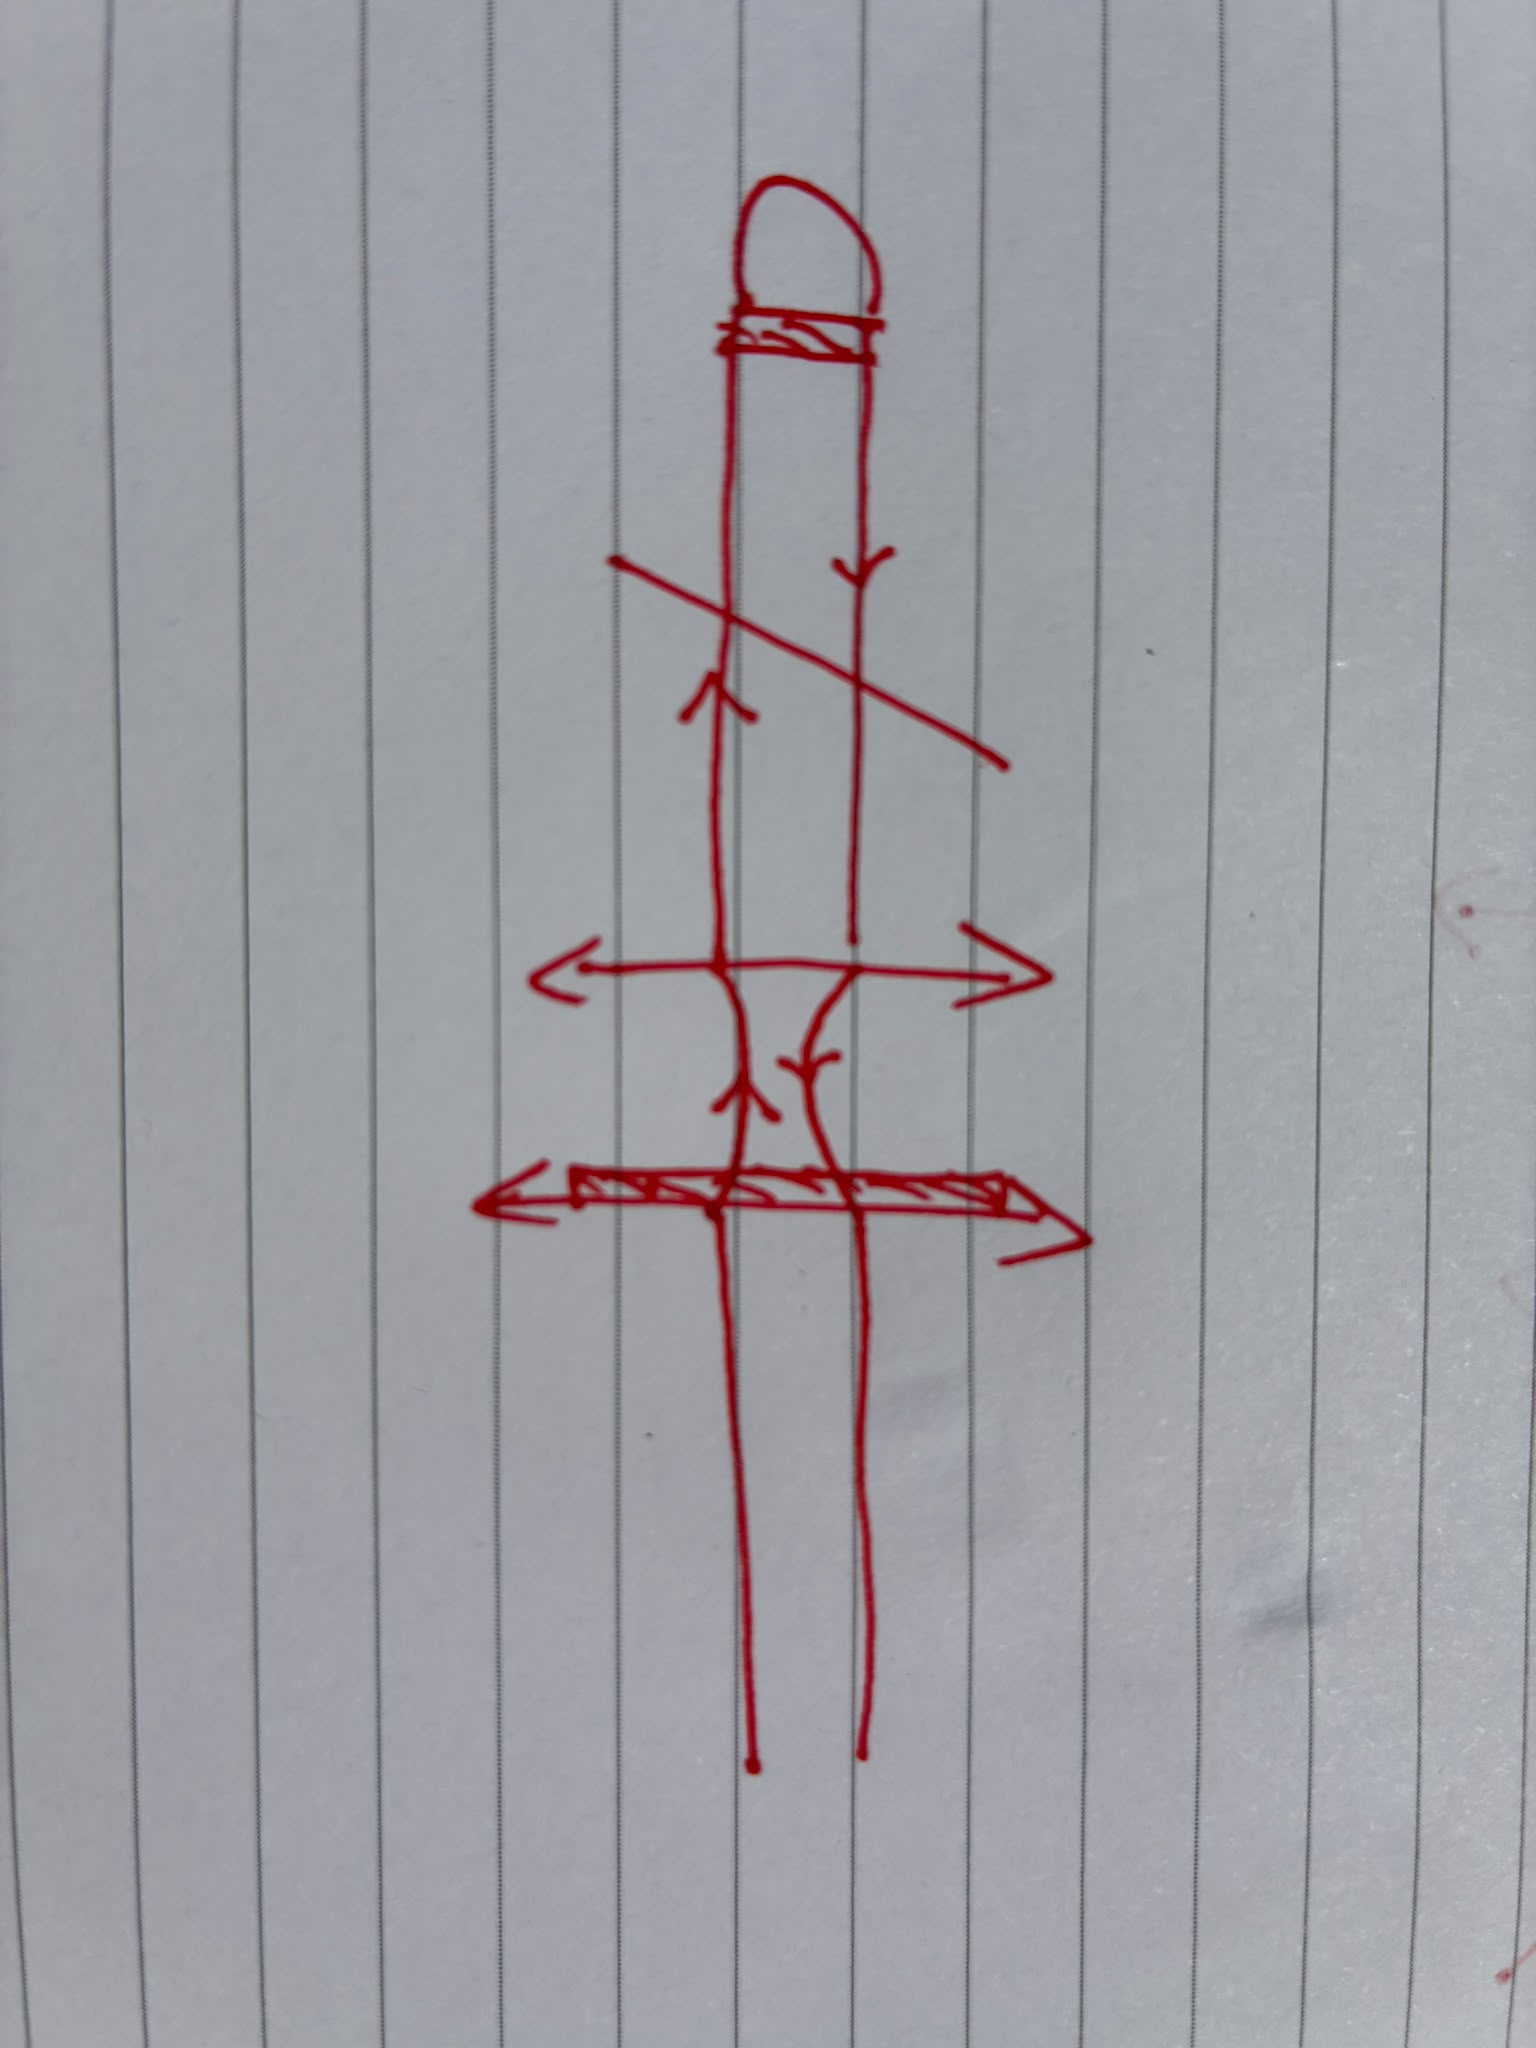
\includegraphics[width=0.5\linewidth, angle=90]{Chapitres/Gas preparation and spin control/images/ECDL_laser.jpeg}
    \caption{MOGlabs External Cavity Diode Laser (ECDL) used for spin manipulation.}
    \label{fig:ecdl-laser}
\end{figure}

\subsection{Raman Transitions}

\subsubsection{Physical Concept}
The second chapter of this thesis focuses on spin manipulation within the $SU(10)$ manifold of $^{87}\text{Sr}$. This operation is realized via a two-photon Raman process driven by two laser beams red-detuned from the $^1S_0 \rightarrow {}^3P_1$ intercombination line.

Controlling the dimension of the effective Hilbert space from 1 to 10 requires independent addressing of individual spin states. The two-photon Rabi frequency $\Omega$ coupling two ground-state sub-levels $\ket{g, m_F}$ and $\ket{g, m_F'}$ through intermediate excited states $\ket{e}$ takes the form:
\begin{equation}
\hbar \Omega = \sum_{e} \frac{\bra{g, m_F'} \vec{d} \cdot \vec{E}_2^* \ket{e} \bra{e} \vec{d} \cdot \vec{E}_1 \ket{g, m_F}}{\Delta_e}
\end{equation}
where $\vec{d}$ is the dipole operator, $\vec{E}_1, \vec{E}_2$ are the electric field amplitudes, and $\Delta_e$ is the single-photon detuning relative to the intermediate state $\ket{e}$.

By applying the TLS, the energy difference between two consecutive spin projections $m_F$ and $m_F+1$ becomes non-linear:
\begin{equation}
\Delta E_{m_F}^{m_F+1} = q(2 m_F + 1) + \beta
\end{equation}
where $q$ parameterizes the quadratic (tensor) light shift and $\beta$ represents the linear Zeeman contribution. This explicit dependence on $m_F$ lifts the energy degeneracy between adjacent transitions, allowing spectral isolation and individual control of any given $m_F \leftrightarrow m_F+1$ pair.

\begin{figure}[H]
    \centering
    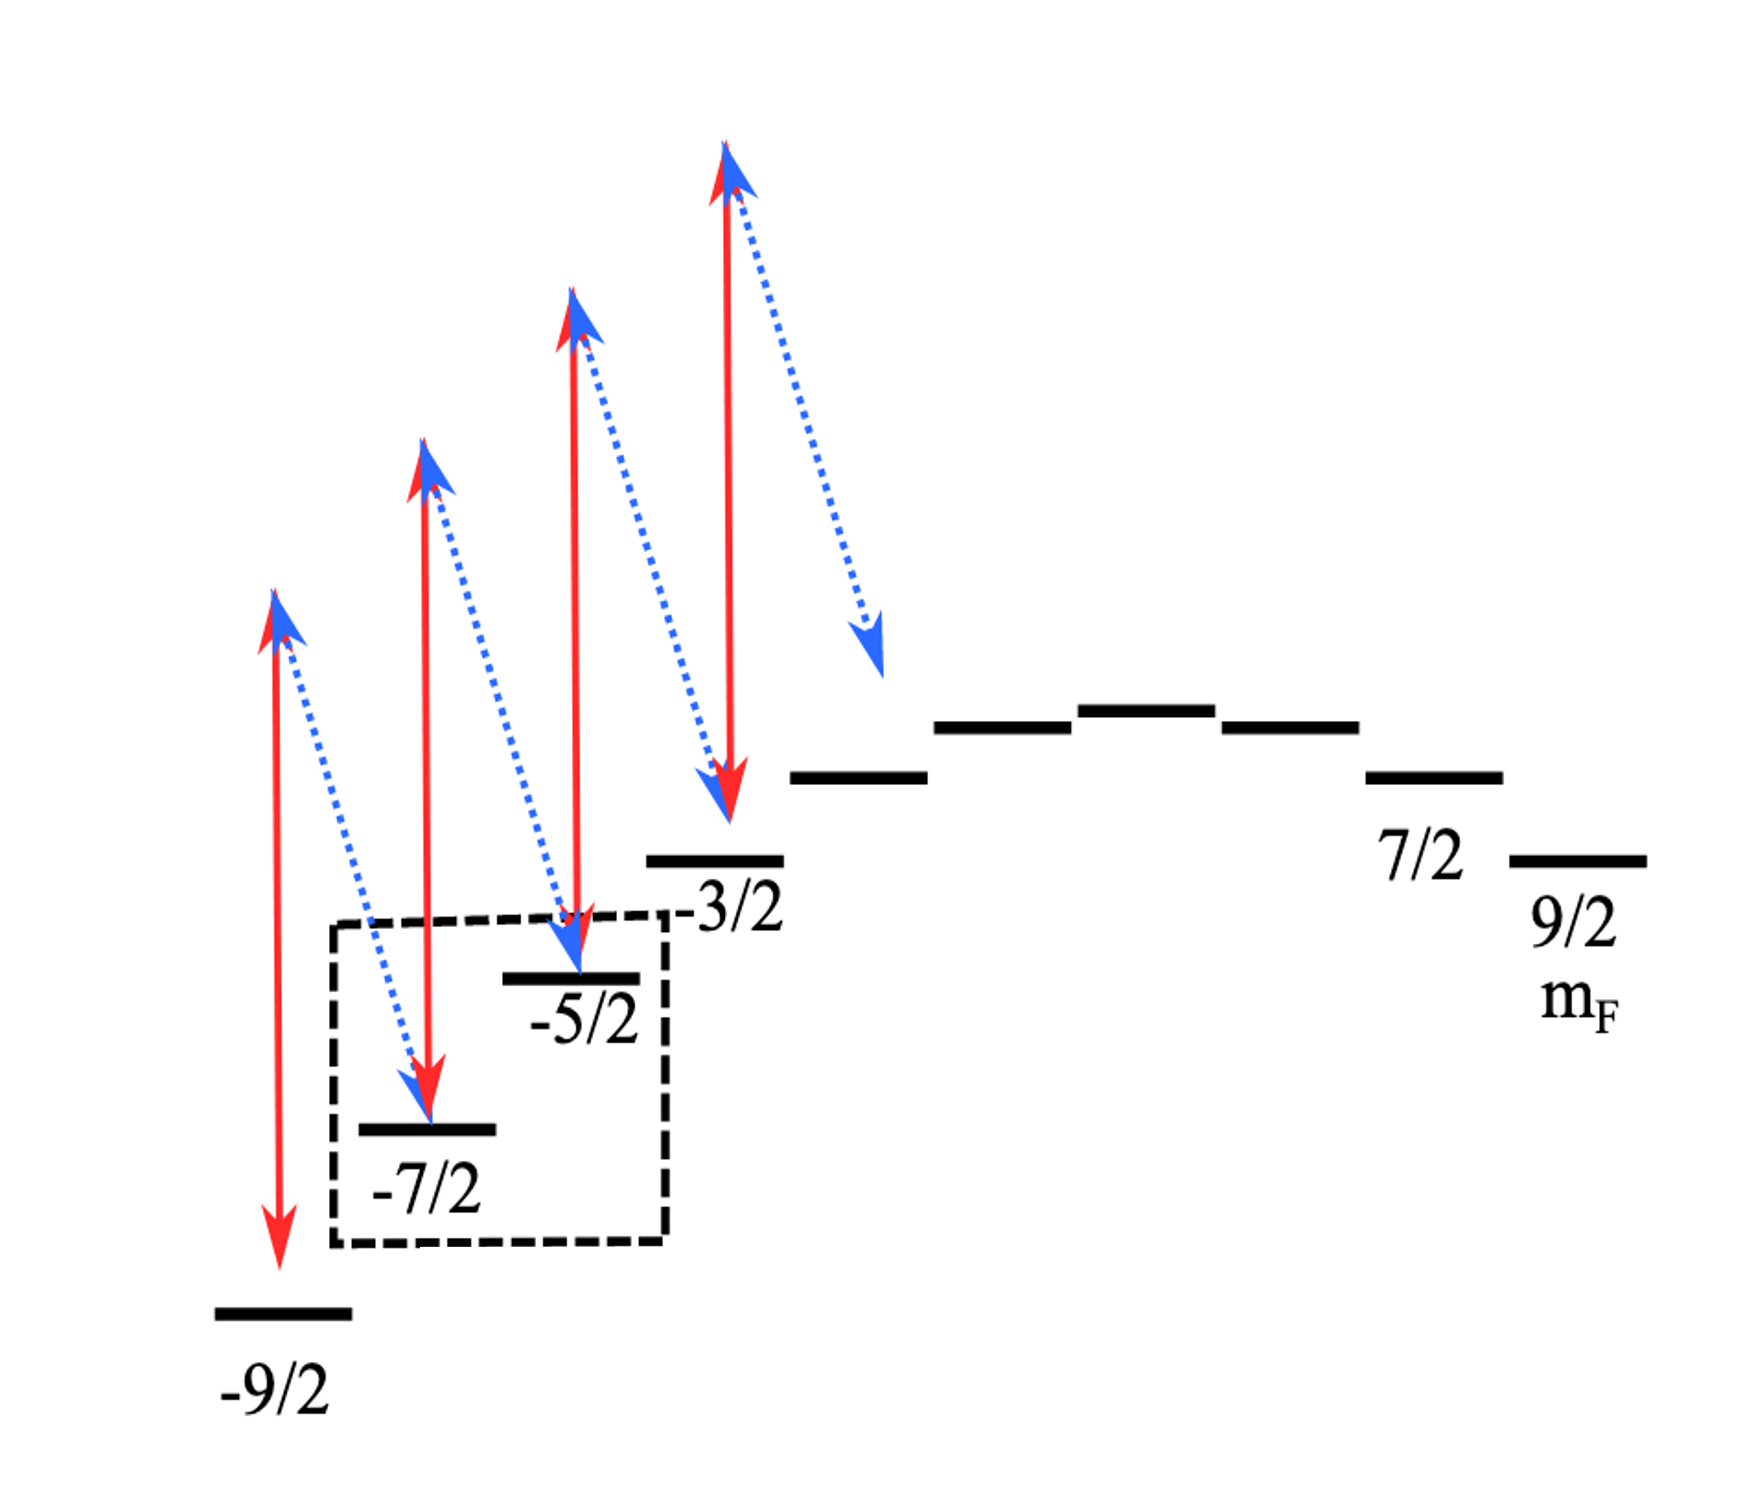
\includegraphics[width=1\linewidth]{Chapitres/Gas preparation and spin control/images/TLS_et_raman.png}
    \caption{Energy level diagram illustrating the Tensorial Light Shift (TLS) and state-selective two-photon Raman transitions.}
    \label{fig:tls-raman-scheme}
\end{figure}

For more details this process is discussed in the second chapter of this thesis and also in the article of the group \cite{Bataille2020}.
\subsubsection{Experimental Setup of the Raman Process}
The two-photon process is driven by two distinct beams: a first beam derived from the "AOM lattice 689" laser (shown in red in Fig.~\ref{fig:raman-transitions}) generates the TLS and supplies the first photon. A second beam, frequency-shifted by the "AOM Raman" (shown in blue), completes the Raman transition. 

This configuration selectively couples a single pair of states—for instance, $\ket{^1S_0, F=9/2, m_F=-7/2} \rightarrow \ket{^1S_0, F=9/2, m_F=-5/2}$—while remaining far off-resonance for all other $m_F$ states. The complete optical path for this operation is detailed in Fig.~\ref{fig:mog-raman}.
The magnetic field is close to zero when the ratio between the two lasers is set $I_R << I_{D}$ since we mostly want to separate the states.

\begin{figure}[H]
    \centering
    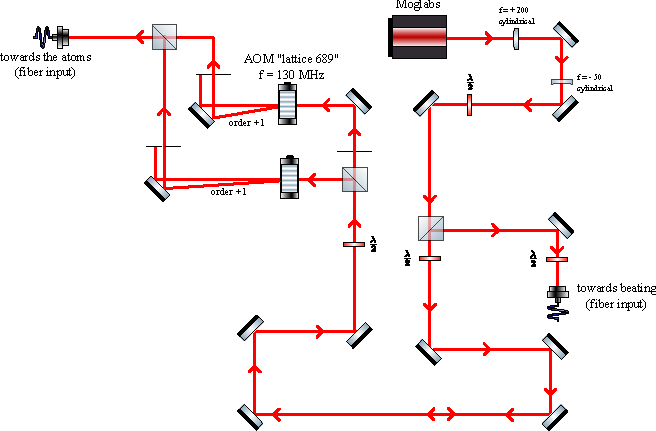
\includegraphics[width=1\linewidth]{Chapitres/Gas preparation and spin control/images/chaine_moglab.pdf}
    \caption{Optical layout of the MOGlabs laser chain configured for two-photon Raman transitions.}
    \label{fig:mog-raman}
\end{figure}

\subsection{Photoassociation}
Chapter 3 investigates photoassociation spectroscopy below the intercombination line. For these measurements, the full power of the laser is sent through the "AOM lattice 689" instead of being split with the Raman AOM.

For the dataset presented in Chapter 3, the optical chain incorporates a custom-built confocal Fabry-Pérot cavity stabilized using the Pound-Drever-Hall (PDH) technique \cite{black_Gas preparation and spin control_2001}, yielding the final setup depicted in Fig.~\ref{fig:raman-transitions}. The beam first passes through an Electro-Optic Modulator (EOM) to generate phase modulation sidebands. A lens with focal length $f = 150~\text{mm}$ mode-matches the beam to the fundamental cavity mode. Upon reflection from the cavity, the light is directed onto a fast photodiode and demodulated with an RF source to produce the PDH error signal.

\begin{figure}[H]
    \centering
    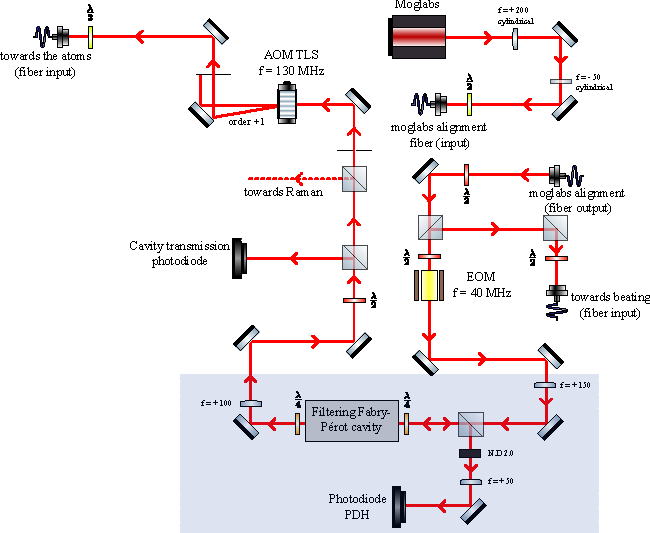
\includegraphics[width=1\linewidth]{Chapitres/Gas preparation and spin control/images/moglab.pdf}
    \caption{Complete optical setup including the Fabry-Pérot cavity and PDH stabilization loop.}
    \label{fig:raman-transitions}
\end{figure}

This cavity filters amplified spontaneous emission (ASE) from the laser source, thereby reducing stray light, minimizing photon-recoil heating.

\subsection{Fabry-Pérot cavity and PDH Locking system}
\subsubsection{Cavity design and assembly}

A primary objective of the cavity injection scheme in our optical setup is to maximize overall transmission for spin manipulation. To achieve this, we constructed a confocal cavity configuration ($d_0 = R_C$, where $d_0$ is the mirror separation and $R_C$ is their radius of curvature), ensuring that all odd transverse modes are degenerate and resonate at the same frequency. If these modes were non-degenerate, off-resonance spatial components would be reflected at the input mirror, thereby reducing the total cavity transmission efficiency.

In addition to the confocal geometry, longitudinal mode resonance requires that the cavity length $d_0$ satisfies the condition:
\begin{equation}
d_0 = n \frac{\lambda}{2}
\label{eq:cavity_resonance}
\end{equation}
where $n$ is an integer and $\lambda$ is the wavelength of the injection laser.

To fulfill these requirements, we selected curved mirrors (\textbf{PD080.31} from PICMA) with a diameter of $D = 4.5 \pm 0.15~\text{mm}$ and a radius of curvature matching $d_0$. The manufacturer specified a nominal mirror transmission of $T_{\text{mirror}} = 1.28\%$, though the effective system performance can be influenced by mechanical mounting constraints.

Proper cavity operation requires the mirrors to be aligned precisely parallel to each other and perpendicular to the optical propagation axis. In our initial implementation (Fig.~\ref{miroirs cav before}), the mirrors were permanently glued into place. However, this approach introduced major technical issues over time: excess glue migrated onto the optical surfaces, degrading overall transmission, while alignment errors during gluing introduced an uncorrected angular tilt relative to the beam axis.

\begin{figure}[H]
    \centering
    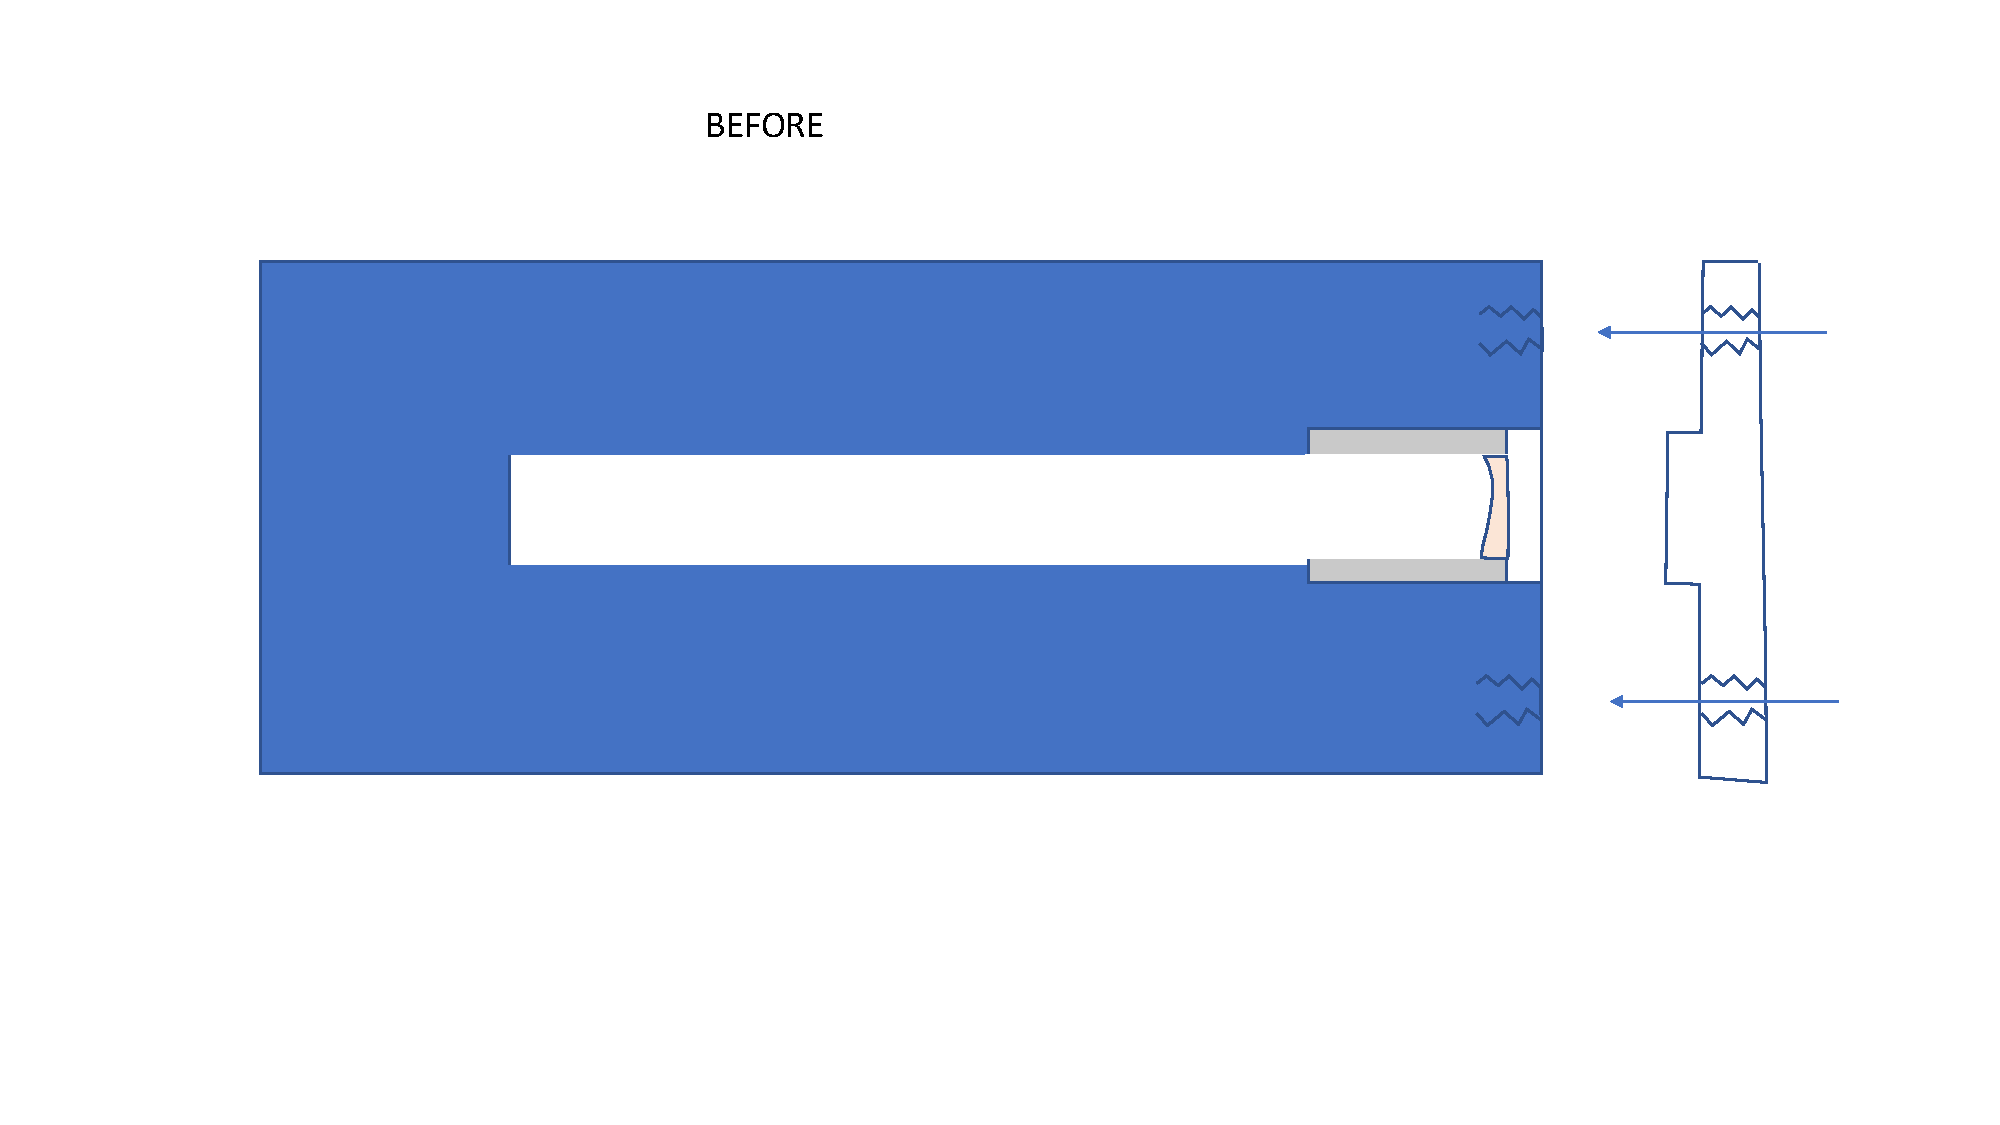
\includegraphics[width=1\linewidth]{Chapitres/Gas preparation and spin control/images/changestoFPcavity.pdf}
    \caption{Initial fixed cavity assembly using glued mirrors, lacking mechanical alignment degrees of freedom.}
    \label{miroirs cav before}
\end{figure}

Because the original design provided no mechanical degrees of freedom to correct these misalignments, we redesigned the mounting mechanism. The updated cavity assembly is presented in Fig.~\ref{miroirs cav after}. In this configuration, three adjustment knobs on a circular outer mount apply controlled pressure against the central cylindrical spacer housing the mirrors, with intermediate washers providing mechanical compliance. This allows for precise tilt control and fine adjustment of the mirror separation.

\begin{figure}[H]
    \centering
    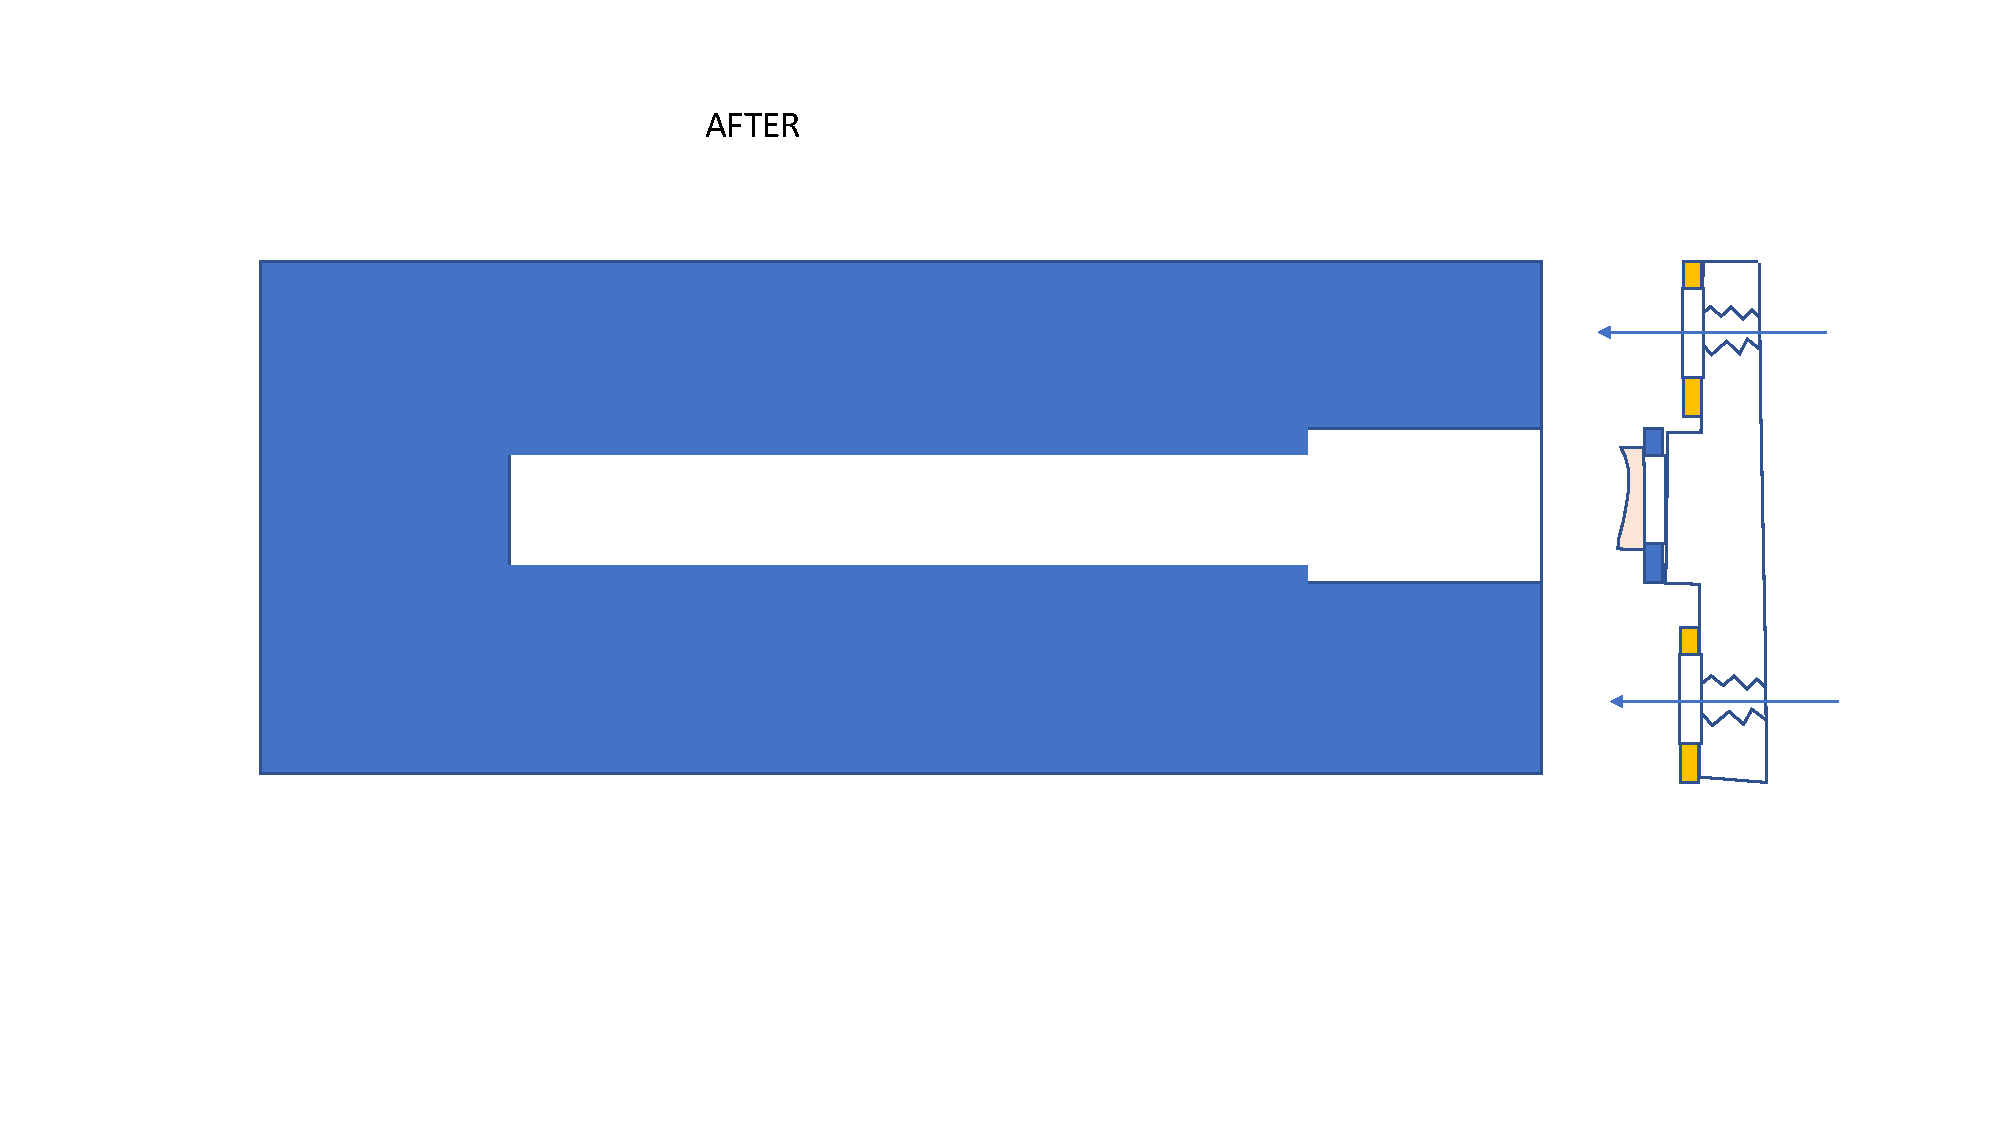
\includegraphics[width=1\linewidth]{Chapitres/Gas preparation and spin control/images/changestoFPcavityAFTER.pdf}
    \caption{Upgraded cavity mount featuring three adjustment screws and compliant washers for precise angular and longitudinal alignment.}
    \label{miroirs cav after}
\end{figure}

Once locked to the injection laser, the optimized cavity achieves a total power transmission efficiency of $T = 0.63$. The Free Spectral Range (FSR) is given by:
\begin{equation}
\text{FSR} = \frac{c}{2 d_0} = 3~\text{GHz}
\end{equation}
with a measured finesse of:
\begin{equation}
\mathcal{F} = \frac{\text{FSR}}{\delta \nu} = 310 \pm 15
\end{equation}
where $\delta \nu$ represents the full width at half maximum (FWHM) of the transmitted resonance peak measured on a photodiode for the odd transverse modes.

\subsubsection{Pound-Drever-Hall locking system and PID controller analysis}

The cavity is frequency-locked to the laser using the Pound-Drever-Hall (PDH) technique, as detailed by Black~\cite{black_Gas preparation and spin control_2001} and schematized in Fig.~\ref{fig:pid}. The scheme utilizes an Electro-Optic Modulator (EOM) to generate sidebands at frequencies $f_0 \pm f_M$ around the optical carrier $f_0$, with a modulation frequency of $f_M = 40.48~\text{MHz}$. The modulated electric field incident on the cavity is expressed as:
\begin{equation}
E_{\text{inc}}^{\text{mod}} \approx E_0 \left[ J_0(\beta) e^{i 2\pi f_0 t} + J_1(\beta) e^{i 2\pi (f_0 + f_M) t} - J_1(\beta) e^{i 2\pi (f_0 - f_M) t} \right]
\end{equation}
where $J_0(\beta)$ and $J_1(\beta)$ are the zeroth- and first-order Bessel functions of the first kind, and $\beta$ is the modulation index.

\begin{figure}[H]
    \centering
    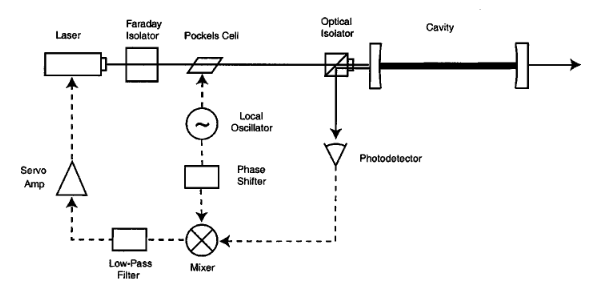
\includegraphics[width=1\linewidth]{Chapitres/Gas preparation and spin control/images/PID_black.png}
    \caption{Schematic of the PDH locking system, extracted from \cite{black_Gas preparation and spin control_2001}.}
    \label{fig:pid}
\end{figure}

The carrier enters the cavity and acquires a steep, frequency-dependent phase shift near resonance, whereas the sidebands are promptly reflected from the input mirror. The interference between the reflected carrier and the sidebands is detected on a fast photodiode, demodulated at $f_M$, and low-pass filtered to extract the dispersive error signal (Fig.~\ref{fig:pdh-error-signal}). The sharp linear slope around resonance provides a robust error signal highly sensitive to the sign of the frequency excursion.
From this graph, one measures a signal-to-noise ratio of \hl{SNR =}. Interestingly, the sideband resonance features were not distinctly visible on the scanning error signal, even when driving the EOM with a high modulation depth to maximize the $J_1/J_0$ ratio.

 \begin{figure}[H]
    \centering
    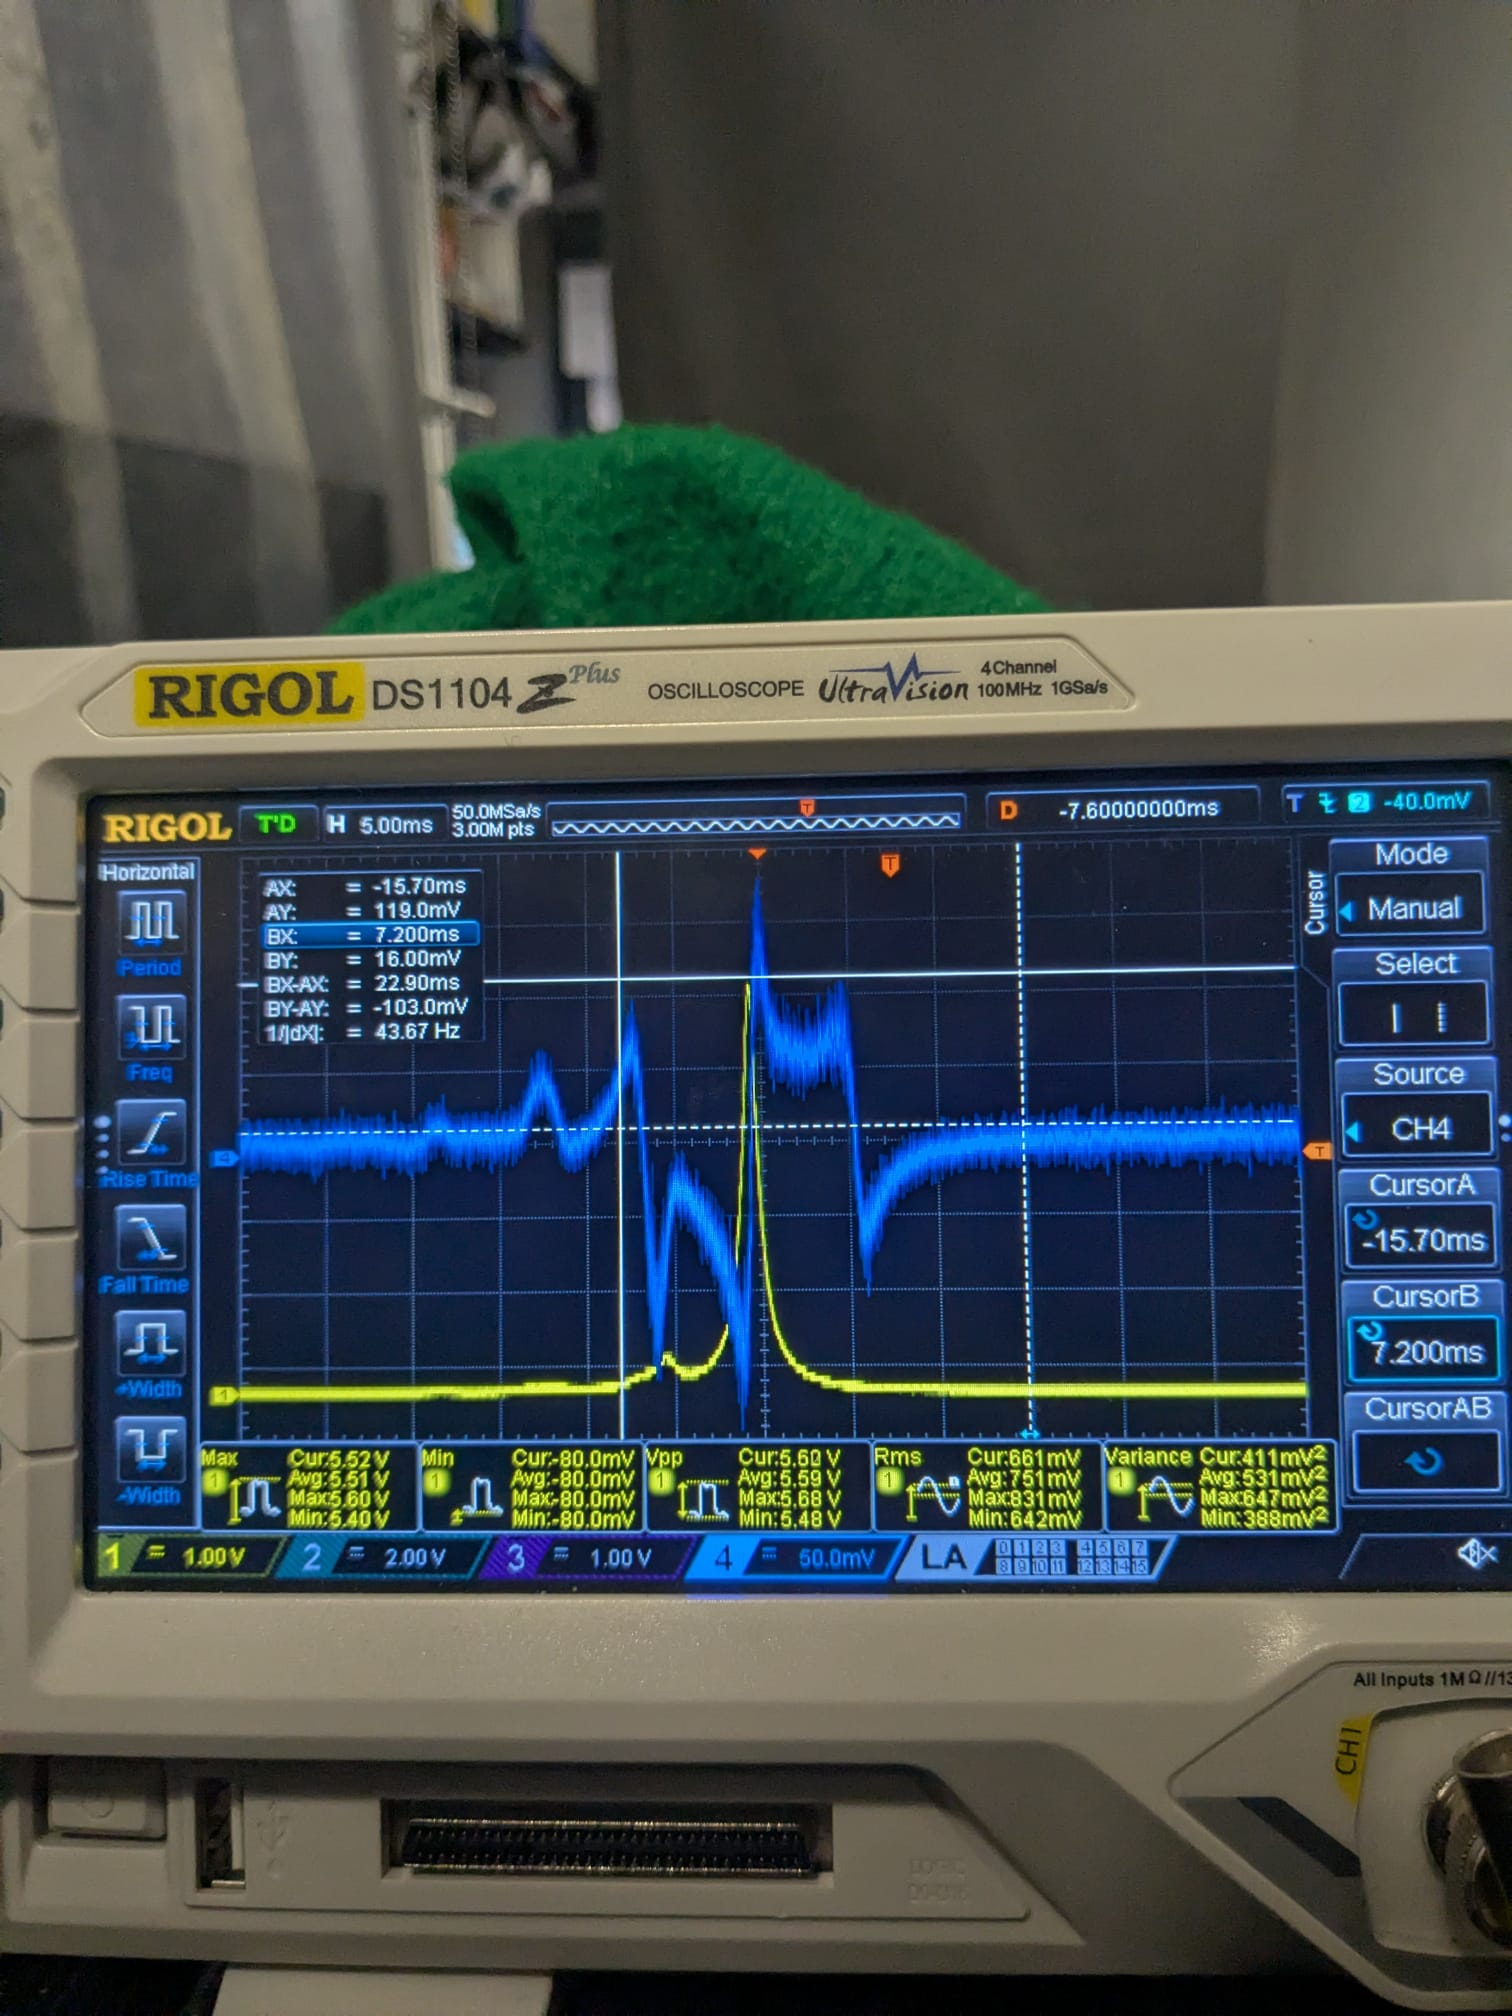
\includegraphics[width=1\linewidth]{Chapitres/Gas preparation and spin control/images/signal pdh.jpg}
    \caption{Typical Pound-Drever-Hall (PDH) error signal obtained by scanning the cavity length across resonance.}
    \label{fig:pdh-error-signal}
\end{figure}

Digital feedback control and noise analysis were implemented primarily using a Red Pitaya STEMlab board. The PID parameters were optimized by injecting a broadband electronic noise signal into the cavity piezo driver and measuring the closed-loop transfer function. As seen in the frequency response plot (Fig.~\ref{fig:analyse_bruit}), operating the system with specific gain values excites mechanical resonances. We interpret the primary peak at $35~\text{kHz}$ as the fundamental mechanical resonance of the piezo actuator, accompanied by other higher-frequency modes.
The noise injection analysis also revealed the low-frequency behavior of the loop. Consequently, the final feedback loop acting on the piezo crystal incorporates a low-pass filter with a cut-off frequency of $f_c = 40~\text{kHz}$, a proportional gain strictly bounded between $1 < K_p < 10$, and an integral gain configured between $0 < K_i < 8~\text{s}^{-1}$.

\begin{figure}[H]
    \centering
    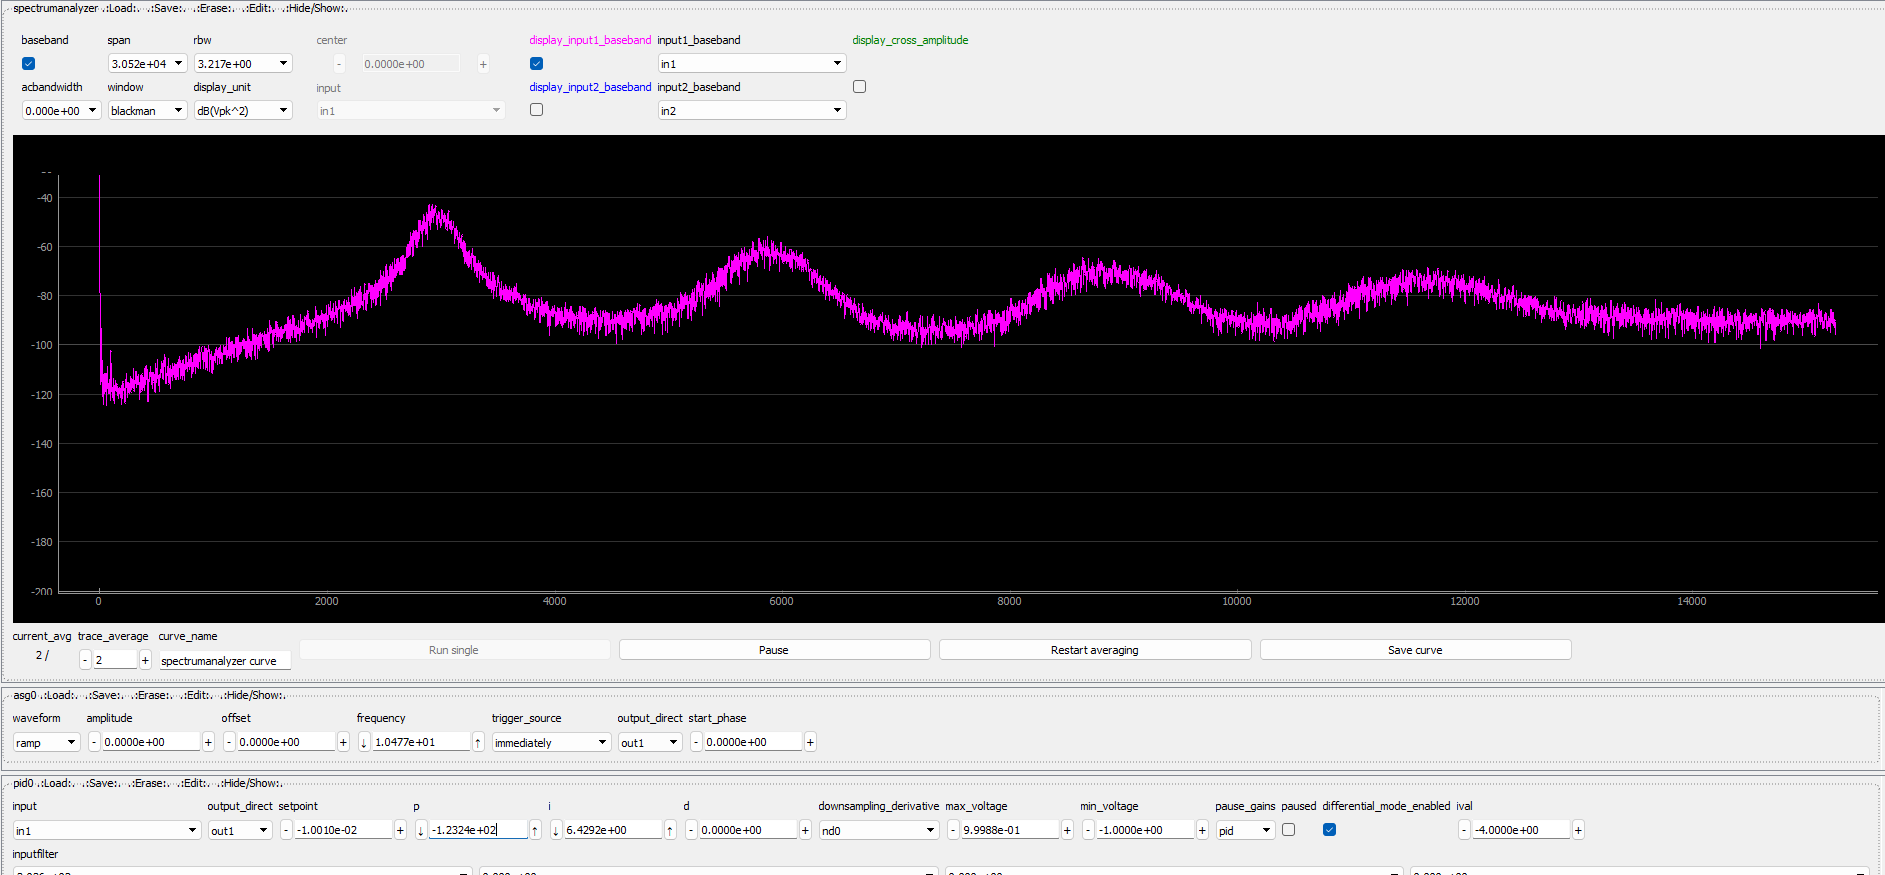
\includegraphics[width=1\linewidth]{Chapitres/Gas preparation and spin control/images/bruits_amplifies.png}
    \caption{Closed-loop noise analysis and mechanical resonance identification using the Red Pitaya.}
    \label{fig:analyse_bruit}
\end{figure}
\section{Spin Measurement Scheme}
Total atom numbers are determined via standard absorption imaging on the broad $^1S_0 \rightarrow {}^1P_1$ transition at $461~\text{nm}$ using a Vortex laser. State-resolved spin detection follows the momentum-transfer ("spin-kick") technique detailed in \cite{bataille_realisation_nodate}.

The measurement sequence proceeds as follows:
\begin{enumerate}
    \item Atoms are illuminated by two counter-propagating laser beams with opposite circular polarizations ($\sigma^+ / \sigma^-$), as illustrated in Fig.~\ref{fig:intro-spin-kick-scheme}(a).
    \item A state-selective pulse tuned to a specific $^1S_0 \rightarrow {}^3P_1$ transition adiabatically transfers targeted spin populations (Fig.~\ref{fig:intro-spin-kick-scheme}(b)).
    \item Each absorption-stimulated emission cycle imparts a coherent $2\hbar k$ momentum kick to the selected $m_F$ state.
    \item Following a time-of-flight (TOF) expansion duration $t=6.6~$ms (set for the gas to stay in camera plane), spatial separation between spin components is observed in the absorption image (Fig.~\ref{fig:intro-spin-kick-scheme}(d)).
\end{enumerate}

Unaddressed spin states remain at the central position of the cloud. In contrast, states subject to the momentum transfer form distinct spatial wavepackets shifted to the left or right depending on the direction of the resonant momentum kick (e.g., $m_F = -3/2$ and $m_F = -7/2$ in Fig.~\ref{fig:intro-spin-kick-scheme}(d)).

To ensure efficient population transfer, the optical pulse sweep rate must satisfy the adiabaticity criterion across the avoided crossing between coupled adiabatic states (Fig.~\ref{fig:intro-spin-kick-scheme}(c)).

\begin{figure}[H]
    \centering
    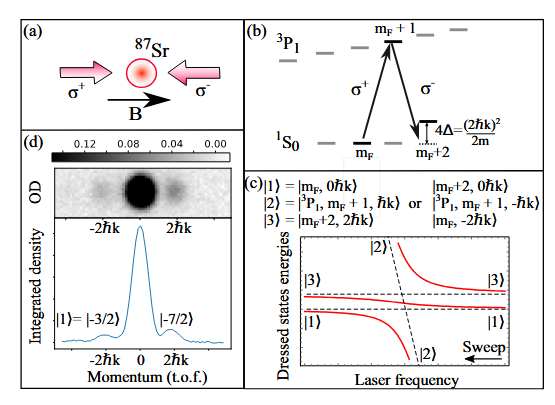
\includegraphics[width=1\linewidth]{Chapitres/Gas preparation and spin control/images/spin_kick_scheme.png}
    \caption{Principle of spin-selective detection via coherent momentum transfer ("spin kick"). (a) Counter-propagating beam geometry. (b) Level scheme. (c) Avoided crossing structure for adiabatic transfer. (d) Resulting TOF absorption image showing spatially separated spin components.}
    \label{fig:intro-spin-kick-scheme}
\end{figure}
